\documentclass[11pt]{article}

\usepackage[english]{babel}
\usepackage[utf8]{inputenc}
\usepackage[T1]{fontenc}
\usepackage{lmodern}
\usepackage{microtype}
\usepackage{amsmath,amssymb,amsthm,mathtools,amscd}
\usepackage[a4paper,margin=1in]{geometry}
\usepackage{parskip}
\usepackage{enumitem}
\usepackage{xcolor}
\usepackage{hyperref}
\usepackage{tikz}
\usetikzlibrary{arrows.meta,positioning,fit,calc,backgrounds}

\hypersetup{colorlinks=true,linkcolor=blue,citecolor=blue,urlcolor=blue}

\newcommand{\R}{\mathbb{R}}
\newcommand{\Z}{\mathbb{Z}}
\newcommand{\Q}{\mathbb{Q}}
\newcommand{\kk}{\Bbbk}
\newcommand{\TAMER}{\textsc{TAMER-OP}}
\newcommand{\multipers}{\textsc{multipers}}
\newcommand{\bbb}[1]{\mathbb{#1}}

\newtheorem{theorem}{Theorem}
\newtheorem{proposition}[theorem]{Proposition}
\newtheorem{lemma}[theorem]{Lemma}
\theoremstyle{definition}
\newtheorem{defn}[theorem]{Definition}
\theoremstyle{remark}
\newtheorem*{remark}{Remark}

%%%%%%%%%%%%%%%%%%%%%%%%%%%%%%%%%%%%%%%%%%%%%%%%%%%%%%%%%%%%%%%%%%%%%%%%%%%%%%%%%%%%%%%%%%%%%%%%%%%%%%%%%%%%%%%%%%
%Some formatting tidbits for margins, paragraphs, and removing orphans

% make widows and orphans rare
\clubpenalty =10000
\widowpenalty =10000

% formatting of paragraphs and separation
\setlength{\parindent}{0pt}
\setlength{\parskip}{5pt plus 1pt}
\setlength{\headheight}{13.6pt}

\setlength\marginparwidth{2.2in}
\setlength\marginparsep{1mm}

%%%%%%%%%%%%%%%%%%%%%%%%%%%%%%%%%%%%%%%%%%%%%%%%%%%%%%%%%

\title{Implementation and Ramifications of TAMER-OP: a Toolkit for Algebraic Module Encodings over $\mathbb{R}^n$ and Other Posets}
\author{Erik Mendes Novak}

\date{\today}

\begin{document}
\maketitle

\newpage
\tableofcontents

\newpage

\section{Introduction}\label{sec:introduction}

Persistent homology is most useful when it converts filtered geometric data into algebraic objects that are simultaneously expressive and computable. In the one-parameter setting these two sides align particularly well. A filtration indexed by a total order gives rise to a persistence module whose structure is rigid enough to admit interval-type decompositions, barcode summaries, and stable diagrammatic invariants \cite{ELZ02,CEH07,CB15,EH10}. In several parameters, however, this balance breaks down. The indexing poset is no longer a chain, a barcode classification is no longer possible in general, and the cost of direct algebraic manipulation grows quickly with the size and geometry of the parameter space \cite{CZ09,Les15,CDSGO16,Oud15}. Multiparameter persistence therefore forces a design choice: one can either work primarily with summary invariants adapted to specific tasks, or one can try to preserve a richer internal algebraic model on which broader constructions remain possible.

The software library \TAMER{} is specifically concerned with the second viewpoint. Its central principle is that the decisive computational move is not a particular invariant, nor a particular data structure for one family of modules, but rather the explicit construction of a finite encoding. Starting from raw data, finite-poset presentations, flange presentations over $\Z^n$, or piecewise-linear presentations over $\R^n$, \TAMER{} first compresses the ambient parameter poset into a finite encoding poset $P$ together with a classifier or encoding map $\pi$. The original object is then represented by a finite-poset module, together with pushed-down presentation data on $P$. Once this finite internal model has been built, the rest of the library's toolkit becomes uniformly available: module morphisms, kernels and cokernels, indicator resolutions, derived functors, rank- and slice-based invariants, serialization, featurization, and visualization can all be performed against the same encoded object. In this sense, encoding is not merely preprocessing, but indeed is the organizing principle of the entire system.

This viewpoint is directly motivated by Miller's theory of tame modules over posets \cite{Mil20}. Miller's framework shows that, under appropriate finiteness hypotheses, several apparently different descriptions of a module are equivalent: finite encodings, indicator presentations by upsets and downsets, and indicator resolutions all express the same controlled form of tameness. That equivalence extends from the theoretical to a strong implementation consequence. Rather than building separate pipelines for geometric data, algebraic summaries, and downstream statistics, one can work to make the encoding step explicit and robust, and then treat the encoded module as the shared internal object from which all later computations are derived.

\TAMER{} consequently accordingly advances three intertwined claims. Firstly, the finite-encoding perspective provides a mathematically coherent bridge between large ambient parameter spaces and finite combinatorial models. Secondly, this bridge is sufficiently explicit to support a unified software architecture that begins with multiple front end representations and data-ingestion pipelines, and ends with exact algebraic, invariant, and statistical workflows. Thirdly, this architecture is practical, as it supports tractable computation on data sets of ordinary scientific scale and is computationally competitive against existing multiparameter persistence libraries where there is implementation overlap.

We are able to accomplish much through \TAMER{} in part due to our language choice. The library is written in \texttt{Julia}, a performant yet high-level programming language, allowing tractability while maintaining clarity and numerical expressiveness.

In the remainder of this thesis, we first introduce the mathematical machinery behind multiparameter persistence and tame modules Then, we overview \TAMER{}, from the front end input, to the encoding step, to downstream computations serialization and visualization. Finally, we benchmark the library to demonstrate its tractability. We hope to demonstrate that nearly every distinctive feature of the library is best understood as more than just an isolated implementation trick, but as a consequence of making the finite encoding step explicit and central.



\section{Multiparameter persistence and its difficulties}\label{sec:background}

Persistent homology begins with a filtered topological object and produces algebra. One chooses an indexing poset, usually a subset of $\R^d$ or $\Z^d$ with the coordinatewise order, and records a vector space at each parameter value together with linear maps along the order relation. In one parameter, this construction leads to a theory with a very strong structure theorem. In several parameters, the same definition still makes sense, but the structure theory changes completely. The purpose of this section is to introduce the basic language carefully and to explain why the multiparameter case resists the sort of complete description that is available in one parameter. Throughout, let $\kk$ be a field.

\subsection{Posets, filtrations, and persistence modules}

The correct indexing objects in persistence theory are partially ordered sets. A poset may be viewed as a category, and a persistence module is then just a functor out of that category.

\begin{defn}[Poset]
A \emph{partially ordered set} is a set $Q$ together with a relation $\leq$ that is reflexive, antisymmetric, and transitive.
\end{defn}

\begin{defn}[A poset as a category]
Given a poset $(Q,\leq)$, one forms a small category, again denoted $Q$, whose objects are the elements of $Q$, and such that there is a unique morphism $q \to q'$ if and only if $q \leq q'$. Composition is forced by transitivity and identity morphisms are forced by reflexivity.
\end{defn}

A category of this form is thin: between any two objects there is at most one morphism. This observation is what allows order theory and homological algebra to interact in persistence.

\begin{defn}[$Q$-module, or persistence module]
Let $Q$ be a poset and let $\mathbf{Vect}_{\kk}$ denote the category of vector spaces over $\kk$. A \emph{$Q$-module} is a covariant functor
\[
M : Q \longrightarrow \mathbf{Vect}_{\kk}.
\]
Equivalently, one specifies a vector space $M(q)$ for each $q \in Q$ and, for each comparable pair $q \leq q'$, a linear map
\[
M(q \leq q') : M(q) \to M(q')
\]
subject to the functoriality relations
\[
M(q \leq q)=\mathrm{id}_{M(q)}, \qquad
M(q \leq q'') = M(q' \leq q'') \circ M(q \leq q')
\]
whenever $q \leq q' \leq q''$.
\end{defn}

A morphism $f : M \to N$ of $Q$-modules is a natural transformation. Concretely, this means that for each $q \in Q$ there is a linear map $f_q : M(q) \to N(q)$ and, for each $q \leq q'$, the square
\[
\begin{CD}
M(q) @>{M(q\leq q')}>> M(q')\\
@V{f_q}VV @VV{f_{q'}}V\\
N(q) @>{N(q\leq q')}>> N(q')
\end{CD}
\]
commutes.

The persistent homology modules arising from filtered topology fit into this framework in the most direct possible way: if $\mathcal{F} : Q \to \mathbf{Top}$ is a filtration, then for each homological degree $i$ one obtains a $Q$-module
\[
H_i(\mathcal{F};\kk) : Q \longrightarrow \mathbf{Vect}_{\kk}
\]
by functoriality of homology.

The category of $Q$-modules inherits the basic exact structure of $\mathbf{Vect}_{\kk}$.

\begin{proposition}[Pointwise abelian structure]
For any small category $\mathcal{C}$, the functor category $\mathrm{Fun}(\mathcal{C},\mathbf{Vect}_{\kk})$ is abelian. In particular, when $\mathcal{C}=Q$ is a poset, kernels, cokernels, images, and coimages are computed pointwise \cite{Mac98,Wei94}.
\end{proposition}

This pointwise abelian structure is the key to computational feasibility. If the indexing poset is finite, then a persistence module is represented by finitely many vector spaces and finitely many structure maps, so abelian constructions reduce to finite linear algebra. If the indexing poset is infinite, the same proposition still holds formally, but it does not provide a usable algorithm. This gap between formal exactness and finite computability is the problem that motivates the encoding viewpoint later in the thesis.

\subsection{The one-parameter scope}

The one-parameter theory is the model initial case. Let $Q$ be $\R$ or $\Z$ with the usual total order. Then persistent homology produces modules indexed by a chain, and that special geometry forces a rigid structure theory.

\begin{defn}[Interval module]
Let $I \subseteq \R$ be an interval. The associated \emph{interval module} $\kk_I$ is defined by
\[
\kk_I(t)=
\begin{cases}
\kk, & t \in I,\\
0, & t \notin I,
\end{cases}
\]
with structure maps equal to the identity whenever both source and target lie in $I$, and equal to the zero map otherwise.
\end{defn}

\begin{theorem}[Barcode decomposition]
Under the usual pointwise-finite and local-finiteness hypotheses from persistence theory, a one-parameter persistence module decomposes as a direct sum of interval modules, uniquely up to isomorphism and reordering of summands \cite{CB15,Oud15}.
\end{theorem}

This theorem explains why barcodes are so effective. In the one-parameter setting they are more than just heuristic pictures, indeed encoding the module itself under the standard finiteness assumptions. Stability theory then shows that the associated persistence diagrams vary continuously under perturbation of the filtered data \cite{ELZ02,CEH07,CDSGO16}. Thus one-parameter persistence enjoys both classification and stability.

That combination does not generalize. It is natural to ask for the same story in several parameters, but already the algebra of the indexing category becomes too rich.

\subsection{What changes in several parameters}

For $d \geq 2$, the standard indexing posets are $\Z^d$ or $\R^d$ with the coordinatewise order
\[
a \leq b \quad \Longleftrightarrow \quad a_i \leq b_i \text{ for all } i.
\]
This change from a chain to a partial order has major consequences. For example, there are now many incomparable pairs. A module is no longer controlled by a single linear progression of births and deaths. Additionally, if one works over $\Z^d$ or $\mathbb{N}^d$, the algebra is equivalent to the algebra of multigraded modules over a polynomial ring.

\begin{proposition}[Algebraic model over $\mathbb{N}^d$]
A persistence module indexed by $\mathbb{N}^d$ is equivalent to an $\mathbb{N}^d$-graded module over the polynomial ring $\kk[x_1,\dots,x_d]$, where multiplication by $x_i$ records the structure map in the $i$th coordinate direction \cite{CZ09,Oud15}.
\end{proposition}

This equivalence is powerful, because it brings in multigraded commutative algebra. It is also, however, the source of the difficulty. The polynomial ring in several variables is not a principal ideal domain, multigraded modules need not decompose into interval modules, and indecomposables occur in families rather than as a discrete list. In particular, the multiparameter theory does not admit a barcode theorem comparable to the one-parameter case \cite{CZ09,Les15}.

So the obstruction is not just that computations become larger. The problem is also structural: in one parameter, the module itself can be packaged into a complete discrete invariant; but, in several parameters, there is in general no analogous finite complete invariant of that simple form.

This has two immediate consequences for computation.

\begin{enumerate}[label=(\roman*)]
    \item One should not expect a universal normal form that is both complete and as easy to manipulate as a barcode.
    \item If one wants to preserve the full algebraic object, rather than only a summary of it, then one needs a different notion of finiteness.
\end{enumerate}

That second point is the central issue addressed by \TAMER{}. The relevant question is not how to force the multiparameter theory back into one-parameter language, but how to represent the module by finite, computable data without dismissing the algebra one later wants to use.

\subsection{What one computes in place of a barcode}

Although there is no complete barcode-like invariant in general, several families of invariants remain useful. They are partial by necessity, each only recording one aspect of the module rather than all of it. We now overview some main ones.

\begin{defn}[Rank invariant]
Let $M$ be a $Q$-module. For each comparable pair $a \leq b$ in $Q$, the \emph{rank invariant} is
\[
\rho_M(a,b) = \operatorname{rank}\bigl(M(a \leq b)\bigr).
\]
\end{defn}

The rank invariant records how much information survives from one parameter value to another. In one parameter it determines the barcode. In several parameters it remains important, but is no longer a complete characterization (different modules may have the same rank invariant).

A second common idea is to probe a multiparameter module along one-dimensional subposets.

\begin{defn}[Restriction to a chain or slice]
If $\lambda : Q' \to Q$ is a monotone map, then the pullback
\[
\lambda^* M := M \circ \lambda
\]
is a $Q'$-module. When $Q'$ is totally ordered, $\lambda^*M$ is an ordinary one-parameter persistence module. Its barcode is then called a \emph{slice barcode} or \emph{fibered barcode}, depending on the context.
\end{defn}

This recovers the successful one-parameter theory on each slice, and it is the basis of tools such as RIVET \cite{LW15,RIVET}. But again, different multiparameter modules can have the same family of one-dimensional restrictions.

There are also dimension-based invariants. The most basic one is the restricted Hilbert function
\[
q \longmapsto \dim_{\kk} M(q).
\]
This records the size of each fiber but not the structure maps between fibers.

A related family comes from chain complexes rather than from a single module. If $C^\bullet$ is a chain or cochain complex of modules on a finite encoding poset, one may define the Euler characteristic function
\[
\chi_C(q) = \sum_t (-1)^t \dim_{\kk} C^t(q).
\]
When $C^\bullet$ arises from filtered topology, this agrees with the alternating sum of the homology dimensions at $q$. In this thesis, when we speak of \emph{Euler invariants}, we mean invariants built from this Euler characteristic function, together with the finite-grid signed measures obtained from it by Mobius inversion. These invariants are useful because they are cheap to evaluate, easy to visualize, and often effective in statistical pipelines, even though they are far from complete.

The essential point is that none of these constructions replaces the module itself. Rank invariants, slice barcodes, Hilbert functions, and Euler characteristic functions are all informative, but each forgets some part of the structure. This is why the central focus of \TAMER{} is not the design of a single invariant, but rather the construction of a finite algebraic model from which many different invariants and constructions can be extracted.

\section{Tameness, finite encodings, and computability}\label{sec:tameness}

The correct response to the loss of barcode classification is to identify a class of modules that still admit finite descriptions and remain amenable to exact algebraic computation. In this thesis that role is played by tame modules in the sense of Miller \cite{Mil20}. We now explore what finite encodings are and why tameness is so important.

\subsection{Finite encodings}

The basic finiteness notion is that a module factors through a finite poset.

\begin{defn}[Finite encoding]
Let $Q$ be a poset and let $M$ be a $Q$-module. A \emph{finite encoding} of $M$ consists of
\begin{enumerate}[label=(\roman*)]
    \item a finite poset $P$,
    \item a monotone map $\pi : Q \to P$, and
    \item a $P$-module $H$ with finite-dimensional stalks,
\end{enumerate}
such that
\[
M \cong \pi^* H = H \circ \pi.
\]
\end{defn}

Here $\pi^*$ denotes pullback along the poset morphism $\pi$.

\begin{defn}[Pullback along a poset morphism]
If $\pi : Q \to P$ is monotone and $H$ is a $P$-module, the \emph{pullback} of $H$ along $\pi$ is the $Q$-module
\[
\pi^*H := H \circ \pi.
\]
Thus
\[
(\pi^*H)(q)=H(\pi(q))
\]
for each $q \in Q$, and the structure map from $q$ to $q'$ is the structure map of $H$ from $\pi(q)$ to $\pi(q')$.
\end{defn}

\begin{proposition}[Exactness of pullback]
For any monotone map $\pi : Q \to P$, the pullback functor
\[
\pi^* : \mathbf{Vect}_{\kk}^{P} \longrightarrow \mathbf{Vect}_{\kk}^{Q}
\]
is exact.
\end{proposition}

\begin{proof}
Kernels, cokernels, and finite direct sums in a functor category are computed pointwise. Pullback by precomposition simply evaluates the $P$-module at $\pi(q)$ instead of at $q$, so exactness is preserved at every stalk.
\end{proof}

A finite encoding is therefore not a lossy statistic. It is an isomorphic re-expression of the module through a finite index category. If $M \cong \pi^*H$, then the algebraic behavior of $M$ is constant on each fiber of $\pi$, and every fiber and structure map of $M$ is recovered from the finite-poset module $H$ together with the map $\pi$.

\subsection{Tame modules and tame morphisms}

With the notion of finite encoding in hand, tameness is simple to state.

\begin{defn}[Tame module]
Let $Q$ be a poset. A $Q$-module $M$ is \emph{tame} if it admits a finite encoding.
\end{defn}

This definition is stronger than merely asking for finite-dimensional fibers or finite-rank structure maps. It requires the entire module to be controlled by finitely many regions of parameter space. That extra strength is exactly what makes it suitable for computation.

There is, however, a subtle categorical point. If one allows all natural transformations between tame modules, kernels and cokernels need not remain finitely encoded. The correct category is obtained by restricting to morphisms that are themselves compatible with a common finite description.

\begin{defn}[Tame morphism]
Let $M$ and $N$ be tame $Q$-modules. A morphism $f : M \to N$ is called \emph{tame} if there exists a common finite constant subdivision, or equivalently a common finite encoding context, in which the component maps of $f$ are constant on each region in the obvious sense \cite{Mil20}.
\end{defn}

\begin{theorem}[Miller]
With tame modules as objects and tame morphisms as morphisms, the resulting category is abelian \cite{Mil20}.
\end{theorem}

This addresses a natural concern. One might worry that finite encodability is too restrictive to support genuine homological algebra. The point of Miller's framework is that this is not the case: the correct category of tame modules is still abelian, so kernels, cokernels, exact sequences, and derived constructions remain available. Recent work of Waas further clarifies that categories of finitely encodable persistence modules have better exact behavior than one might first expect, reinforcing the view that finite encodability is a mathematically natural rather than ad hoc hypothesis \cite{Waa24}.

Thus, the word tame should not be read as a purely artificial restriction imposed for software convenience. It identifies the point at which an ambient persistence module can be represented by finite data without collapsing to a summary invariant that loses information. For the purposes of \TAMER{}, tameness is the hypothesis that makes it possible to keep the module, rather than discard it, and still work computationally. 

\subsection{Upsets, downsets, and fringe presentations}

Finite encodings are one language for tameness. Another is given by indicator modules attached to order-theoretic regions.

\begin{defn}[Upsets and downsets]
Let $Q$ be a poset.
\begin{enumerate}[label=(\roman*)]
    \item An \emph{upset} is a subset $U \subseteq Q$ such that $q \in U$ and $q \leq q'$ imply $q' \in U$.
    \item A \emph{downset} is a subset $D \subseteq Q$ such that $q' \in D$ and $q \leq q'$ imply $q \in D$.
\end{enumerate}
For $q \in Q$, the corresponding principal upset and principal downset are
\[
\uparrow q = \{q' \in Q : q \leq q'\}, \qquad
\downarrow q = \{q' \in Q : q' \leq q\}.
\]
\end{defn}

\begin{defn}[Indicator modules]
To an upset $U \subseteq Q$ one associates the \emph{upset indicator module} $\kk\{U\}$, defined by
\[
\kk\{U\}(q)=
\begin{cases}
\kk, & q \in U,\\
0, & q \notin U,
\end{cases}
\]
with the evident structure maps. Dually, a downset $D$ determines a \emph{downset indicator module} $\kk\{D\}$.
\end{defn}

On a finite poset, principal upset indicators play the role of indecomposable projective modules, and principal downset indicators play the role of indecomposable injective modules. This is why they are the correct basic pieces for exact algebra on finite posets.

\begin{defn}[Finite fringe presentation]
A \emph{finite fringe presentation} of a $Q$-module $M$ consists of a morphism
\[
\varphi : \bigoplus_{i=1}^m \kk\{U_i\} \longrightarrow \bigoplus_{j=1}^r \kk\{D_j\}
\]
from a finite direct sum of upset indicator modules to a finite direct sum of downset indicator modules such that $M \cong \operatorname{im}(\varphi)$ \cite{Mil20}.
\end{defn}

This presentation language is one of the key bridges between geometry and algebra in the library. Upsets encode where generators are born and persist upward in the order; downsets encode where relations become enforced; and the matrix of $\varphi$ records how these pieces interact.

\subsection{Why encoding is the right answer}

The key fact is that tameness admits several equivalent finite descriptions.

\begin{theorem}[Syzygy theorem, after Miller]
For a module over a poset, the following finiteness conditions are equivalent: existence of a finite encoding, existence of a finite fringe presentation, and existence of finite resolutions by indicator modules \cite{Mil20}.
\end{theorem}

This theorem explains why encoding is the right computational answer to the difficulties of multiparameter persistence. We describe three consequences of it now.

Firstly, it says that one does not need to choose between a geometric region picture, a presentation by births and deaths, and a homological description by resolutions. For tame modules, these are different finite views of the same object.

Secondly, it explains what is gained by encoding. We do not package a multiparameter module back into one clean barcode, because that is impossible in general. Instead, we pass to a finite poset on which the module is represented exactly by finite data. Once that finite representation has been constructed, one can carry out actual algebra: kernels, cokernels, change-of-poset operations, indicator resolutions, and derived functor calculations. Invariants such as rank functions, slice barcodes, Hilbert functions, Euler characteristic functions, and their associated signed measures are then extracted from this finite model, rather than substituted for it.

Thirdly, it explains why this approach does not lose information in the sense relevant to the library. The encoded module on the finite poset is not a secondary summary attached to the original module, but rather the finite algebraic object through which the original module is being represented. The purpose of the encoding step is therefore not compression for its own sake. It is to move from an ambient indexing space that is too large for direct exact computation to a finite model on which exact computation is possible.

This is the perspective adopted throughout the rest of the thesis. The next section therefore begins with the architecture of the encoding-centered system itself, because once the encoded finite-poset module has been built, the rest of the library follows from that choice.

\section{Overview of \TAMER{} as an encoding-centered system}\label{sec:system-overview}

The previous section explained why finite encodings are mathematically legitimate and computationally necessary.  This section explains how that idea informs the organization of \TAMER{}.  We identify the stable mathematical interfaces that the implementation is built around; these are arranged so that many front-end objects feed a single encoding step, and that encoding step in turn feeds many downstream computations.

At the highest level, the library is organized around the composite workflow
\[
\mathcal{I}
\xrightarrow{\ \mathsf{prepare}\ }
\mathcal{P}
\xrightarrow{\ \mathsf{encode}\ }
\mathcal{E}
\xrightarrow{\ \mathsf{analyze}\ }
\mathcal{O},
\]
where:
\begin{itemize}[leftmargin=1.5em]
    \item $\mathcal{I}$ denotes raw inputs, such as data files, point clouds, graphs, images, or already structured presentation objects;
    \item $\mathcal{P}$ denotes pre-encoding mathematical objects, such as finite fringe modules, flanges over $\mathbb{Z}^n$, PL or box presentations over $\mathbb{R}^n$, and labeled cell complexes produced by ingestion;
    \item $\mathcal{E}$ denotes finite encodings, represented concretely by a finite poset together with an encoded module and the maps needed to interpret it back in the ambient parameter space; and
    \item $\mathcal{O}$ denotes downstream outputs, including categorical constructions, derived functors, invariants, feature vectors, serialized artifacts, and visual objects.
\end{itemize}

The crucial middle object $\mathcal{E}$ is what the codebase packages as an \texttt{EncodingResult}.  Stripping away software metadata, the mathematical content of such an object is the tuple
\[
(P,M,\pi,H).
\]
Here $P$ is a finite encoding poset, $M$ is a finite-poset module on $P$, $\pi$ is the classifier or encoding map from the ambient domain to $P$, and $H$ is a pushed-down fringe presentation when such a presentation is available.  Not every later calculation uses all four pieces, but together they constitute the canonical object available to the rest of the system.

This packaging is contextually important: the encoding step does not merely return a poset and forget how it arose; it returns a finite module, a mechanism for point location in the original parameter space, and enough provenance to support comparison, serialization, and visualization. From the user-facing point of view, this is the moment at which a raw front end object becomes a reusable algebraic object.

Figure~\ref{fig:system-overview} summarizes the resulting architecture.

\begin{figure}[h]
\centering
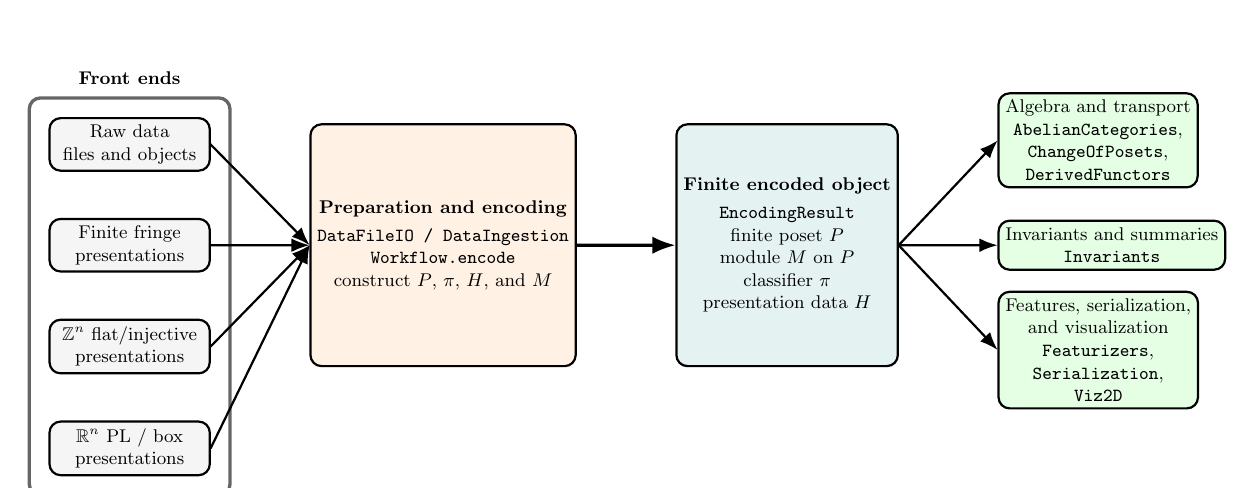
\begin{tikzpicture}[
    >=Latex,
    scale=0.74,
    transform shape,
    node distance=8mm and 10mm,
    every node/.style={font=\small},
    src/.style={rounded corners, draw, thick, align=center, minimum width=2.75cm, minimum height=0.8cm, fill=gray!8},
    stage/.style={rounded corners, draw, thick, align=center, minimum width=3.8cm, minimum height=1.0cm, fill=orange!10},
    outbox/.style={rounded corners, draw, thick, align=center, minimum width=3.0cm, minimum height=0.82cm, fill=green!10},
    layer/.style={rounded corners, draw=black!60, very thick, inner sep=7pt}
]

\node[src] (raw) {Raw data\\files and objects};
\node[src, below=of raw] (finite) {Finite fringe\\presentations};
\node[src, below=of finite] (flange) {$\mathbb{Z}^n$ flat/injective\\ presentations};
\node[src, below=of flange] (pl) {$\mathbb{R}^n$ PL / box\\presentations};
\node[layer, fit=(raw)(finite)(flange)(pl), label={[yshift=0.2em]above:\textbf{Front ends}}] {};

\node[stage, right=17mm of finite, minimum height=4.15cm] (encode) {
\textbf{Preparation and encoding}\\[0.3em]
\texttt{DataFileIO / DataIngestion}\\
\texttt{Workflow.encode}\\
construct $P$, $\pi$, $H$, and $M$
};

\node[stage, right=17mm of encode, minimum height=4.15cm, fill=teal!10] (result) {
\textbf{Finite encoded object}\\[0.3em]
\texttt{EncodingResult}\\
finite poset $P$\\
module $M$ on $P$\\
classifier $\pi$\\
presentation data $H$
};

\node[outbox, right=17mm of result, yshift=18mm] (alg) {Algebra and transport\\\texttt{AbelianCategories},\\\texttt{ChangeOfPosets},\\\texttt{DerivedFunctors}};
\node[outbox, right=17mm of result] (inv) {Invariants and summaries\\\texttt{Invariants}};
\node[outbox, right=17mm of result, yshift=-18mm] (feat) {Features, serialization,\\and visualization\\\texttt{Featurizers},\\ \texttt{Serialization},\\ \texttt{Viz2D}};

\draw[->, thick] (raw.east) -- (encode.west);
\draw[->, thick] (finite.east) -- (encode.west);
\draw[->, thick] (flange.east) -- (encode.west);
\draw[->, thick] (pl.east) -- (encode.west);
\draw[->, very thick] (encode.east) -- (result.west);
\draw[->, thick] (result.east) -- (alg.west);
\draw[->, thick] (result.east) -- (inv.west);
\draw[->, thick] (result.east) -- (feat.west);

\end{tikzpicture}
\caption{A system-level view of \TAMER.  Multiple front ends are normalized into a single encoded object, and all later computation branches from that encoded object rather than from the original ambient representation.}
\label{fig:system-overview}
\end{figure}

The diagram is purposefully thin in the center but branched in input and output.  The left side is diverse because the library is intended to accept front-end objects in the form most natural to their source.  The middle is narrow because there is only one conceptual move that matters: build a finite encoding.  The right side branches again because, once the encoded object exists, many different computational goals can be pursued from the same internal representation.

This thin diagrammatic section characterizing encoding identifies the precise place at which the computational problem changes style. Before encoding, one is still dealing with ambient parameter spaces, geometric representations, filtration choices, and presentation-specific subtleties.  After encoding, one is dealing with a finite-poset module.  The post-encoding world is therefore uniform even though the pre-encoding world is intentionally heterogeneous.

This is also the main mathematical reason that \TAMER{} can do things that are awkward or impossible for existing libraries, which are generally built around architectures that prioritize only summaries and invariants.  Once an actual encoded module has been retained, one may compute kernels, cokernels, equalizers, pushouts, projective and injective approximations, derived functors, and comparison transports before one ever decides which invariant or feature vector to extract.  The encoded module is therefore not just a transient intermediate artifact, but the central object around which the rest of the pipeline is organized.

The rest of the thesis will follow the flow of figure \ref{fig:system-overview}, with the next chapter describing pre-encoding objects and data interfaces.


\section{Pre-encoding objects and data interfaces}\label{sec:pre-encoding}

Sections~\ref{sec:background} and~\ref{sec:tameness} introduced the mathematical reason that a finite encoding should exist and should be the object on which exact computation is carried out.  Before one can build such an encoding, however, one needs a finite front end description of the module to be encoded.  This chapter describes the principal front ends accepted by \TAMER{}.

The guiding principle is as follows: the library is intentionally permissive about the form in which a module is first described, but intentionally strict about the object on which later algebra is done.  On the input side, one may begin with a module already indexed by a finite poset, with a \(\mathbb{Z}^n\)-presentation adapted to finitely determined modules, with a piecewise-linear presentation over \(\R^n\), or with raw topological data from which such a presentation can be constructed.  On the output side of the encoding step there is only the working language of a module on a finite encoding poset.

\subsection{Finite-poset presentations: finite fringe presentations and indicator data}

The simplest front end occurs when the indexing poset is already finite.  In that case no geometric compression is needed to obtain a finite combinatorial object, and the basic question is only how to package the module in a form that is easy to manipulate and easy to compare with later encoded outputs.

Let \(P\) be a finite poset.  As in Section~\ref{sec:tameness}, an upset \(U \subseteq P\) determines an indicator module \(\kk\{U\}\), and a downset \(D \subseteq P\) determines an indicator module \(\kk\{D\}\).  Since \(P\) is finite, these indicator modules are themselves finite diagrams of finite-dimensional vector spaces.

\begin{defn}[Finite fringe presentation on a finite poset]
	Let \(P\) be a finite poset and let \(\kk\) be a field.  A \emph{finite fringe presentation} on \(P\) consists of finitely many upsets \(U_1,\dots,U_m\subseteq P\), finitely many downsets \(D_1,\dots,D_r\subseteq P\), and a morphism
	\[
	\varphi : \bigoplus_{i=1}^m \kk\{U_i\}\longrightarrow \bigoplus_{j=1}^r \kk\{D_j\},
	\]
	with the associated module defined as
	\[
	M:=\operatorname{im}(\varphi).
	\]
	Equivalently, once bases are chosen on the one-dimensional indicator summands, the presentation is specified by a matrix
	\[
	\Phi\in \kk^{r\times m}
	\]
	subject to the support condition that \(\Phi_{ji}=0\) whenever \(U_i\cap D_j=\varnothing\).
\end{defn}

The matrix description is especially concrete on a finite poset.  For each vertex \(p\in P\), define the active column and row sets
\[
I(p)=\{i\in\{1,\dots,m\}:p\in U_i\},
\qquad
J(p)=\{j\in\{1,\dots,r\}:p\in D_j\}.
\]
Evaluating the presentation at \(p\) yields a linear map
\[
\varphi_p : \kk^{I(p)}\longrightarrow \kk^{J(p)}
\]
whose matrix is the submatrix \(\Phi_{J(p),I(p)}\).  Thus the fiber at \(p\) is
\[
M(p)=\operatorname{im}(\varphi_p),
\qquad
\dim_\kk M(p)=\operatorname{rank}(\Phi_{J(p),I(p)}).
\]
In other words, the module is read off from the same finite matrix together with the membership pattern of each vertex in the chosen upsets and downsets.

This front end matters for two central reasons.  Firstly, it is the cleanest correctness model in the whole library.  When the user already knows the finite indexing poset, there is no mystery with the encoding; all later kernels, cokernels, Hom, Ext, and invariant computations can be checked directly against this finite presentation.  Secondly, finite fringe presentations are also the natural output of the encoding step, not just merely one among many input formats.  The point of encoding is precisely to replace a module on a large poset by a finite-poset module or, equivalently, by a finite fringe presentation on a finite region poset.  For that reason the finite fringe language is both a front end description and the simplest model of the finite encoding.

\subsection{$\mathbb{Z}^n$ front end: flange presentations and finitely determined data}

The next front end is adapted to modules over \(\mathbb{Z}^n\) with the coordinatewise order.  This is the natural discrete setting for many multifiltration constructions, and it is also the setting in which the connection with multigraded commutative algebra is most direct \cite{CZ09}.  A \(\mathbb{Z}^n\)-module is a functor from the poset category \(\mathbb{Z}^n\) to vector spaces, equivalently a multigraded representation with structure maps in the positive coordinate directions.

A particularly important class is formed by finitely determined modules.

\begin{defn}[Finitely determined \(\mathbb{Z}^n\)-module]
	A \(\mathbb{Z}^n\)-module \(M\) is \emph{finitely determined} if there exists \(a\in \mathbb{Z}^n\) such that for every \(b\geq a\) and every standard basis vector \(e_i\), the structure map
	\[
	M(b\leq b+e_i) : M(b)\longrightarrow M(b+e_i)
	\]
	is an isomorphism.
\end{defn}

This condition says that, sufficiently far in the positive orthant, the module stops changing in any essential way.  It is the discrete analogue of eventual constancy on regions, and it is one of the standard hypotheses under which finite descriptions become possible.

Miller's theory packages these modules using \emph{flats} and \emph{injectives}.  Fix a subset \(\tau\subseteq \{1,\dots,n\}\), thought of as a set of free coordinate directions, and a lattice point \(b\in \mathbb{Z}^n\).  The corresponding flat and injective regions are
\[
F_{\tau,b}=\{a\in \mathbb{Z}^n: a_i\geq b_i\text{ for every }i\notin \tau\},
\]
\[
E_{\tau,b}=\{a\in \mathbb{Z}^n: a_i\leq b_i\text{ for every }i\notin \tau\}.
\]
The coordinates in \(\tau\) are unrestricted.  Thus principal upsets and principal downsets occur as the special case \(\tau=\varnothing\), while more general choices of \(\tau\) allow one to model affine coordinate flats in the sense used in Miller's \(\mathbb{Z}^n\)-theory \cite{Mil20}.

\begin{defn}[Flange presentation]
	A \emph{flange presentation} over \(\mathbb{Z}^n\) consists of finitely many flats \(F_1,\dots,F_m\), finitely many injectives \(E_1,\dots,E_r\), and a matrix
	\[
	\Phi\in \kk^{r\times m}
	\]
	with the support condition \(\Phi_{ji}=0\) whenever \(F_i\cap E_j=\varnothing\).  It presents the module
	\[
	M:=\operatorname{im}\!\left(\bigoplus_{i=1}^m \kk\{F_i\}\longrightarrow \bigoplus_{j=1}^r \kk\{E_j\}\right).
	\]
\end{defn}

The local behavior is parallel to the finite fringe case.  For a lattice point \(g\in\mathbb{Z}^n\), let
\[
I(g)=\{i:g\in F_i\},\qquad J(g)=\{j:g\in E_j\}.
\]
Then the fiber \(M(g)\) is the image of the submatrix \(\Phi_{J(g),I(g)}\), so fiber dimensions and local maps are determined by the active flats and injectives at \(g\).  What changes, compared to the finite-poset case, is that the ambient poset is infinite.  The flange presentation therefore serves as a compact input language whose membership predicates can be evaluated anywhere in \(\mathbb{Z}^n\), but which is intended to be encoded before more substantial algebra is done.

\subsection{$\mathbb{R}^n$ front-end: PL fringes and box presentations}

For modules over \(\mathbb{R}^n\), one needs a geometric version of the same idea.  The relevant inputs are piecewise-linear upsets and downsets, represented by finite polyhedral data.  This is the correct front end for modules whose behavior changes along finitely many polyhedral boundaries, and it is also the natural setting for geometric constructions arising from stratified topology and sheaf-theoretic viewpoints on persistence \cite{KS18,Mil23}.

\begin{defn}[PL upset and PL downset]
	A \emph{PL upset} in \(\mathbb{R}^n\) is an upward-closed subset that is a finite union of convex polyhedra.  A \emph{PL downset} is defined dually as a downward-closed finite union of convex polyhedra.
\end{defn}

The front end presentation is then the direct real-parameter analogue of a fringe presentation.

\begin{defn}[PL fringe presentation]
	A \emph{PL fringe presentation} over \(\mathbb{R}^n\) consists of finitely many PL upsets \(U_1,\dots,U_m\subseteq\mathbb{R}^n\), finitely many PL downsets \(D_1,\dots,D_r\subseteq\mathbb{R}^n\), and a matrix
	\[
	\Phi\in \kk^{r\times m}
	\]
	with \(\Phi_{ji}=0\) whenever \(U_i\cap D_j=\varnothing\).  The associated module is again the image of the induced morphism
	\[
	\bigoplus_{i=1}^m \kk\{U_i\}\longrightarrow \bigoplus_{j=1}^r \kk\{D_j\}.
	\]
\end{defn}

At a point \(x\in\mathbb{R}^n\), one evaluates the same active-set construction as before,
\[
I(x)=\{i:x\in U_i\},\qquad J(x)=\{j:x\in D_j\},
\]
and the fiber is computed from the submatrix \(\Phi_{J(x),I(x)}\).  Thus the formal algebra is unchanged, with change happening in the geometry of membership and intersection.  In the real setting, a correct implementation must be able to decide whether a point lies in one of the finitely many prescribed polyhedral regions and must be able to identify the induced constant regions of the presentation.

An important specialization is the axis-aligned box backend.  Here one restricts to upsets and downsets of the form
\[
U_{\ell}=\{x\in\mathbb{R}^n:x_i\geq \ell_i\text{ for all }i\},
\qquad
D_u=\{x\in\mathbb{R}^n:x_i\leq u_i\text{ for all }i\}.
\]
This format covers a large and practically relevant class of examples. Additionally, and importantly, they admit a much more direct encoding procedure, covered in the next section. So, ultimately, the polyhedral front end is mathematically more general, while the box front end is algorithmically much simpler, and the library supports both.

\subsection{Raw data, filtrations, and labeled cell complexes}

Not every user begins with a presentation by upsets and downsets.  In topological data analysis the more common starting point is raw data together with a rule for assigning parameter values to cells, simplices, edges, or vertices.  For this reason \TAMER{} includes a data-ingestion layer whose role is to convert raw data into one of the presentation objects discussed above, usually by way of a labeled cell complex.

\begin{defn}[Labeled cell complex]
	Let \(K\) be a finite cell complex.  A \emph{labeled cell complex} over a poset \(Q\) is the data of a grade
	\[
	\deg(\sigma)\in Q
	\]
	for each cell \(\sigma\) of \(K\), subject to the monotonicity condition that if \(\tau\) is a face of \(\sigma\), then
	\[
	\deg(\tau)\leq \deg(\sigma).
	\]
	Equivalently, the chain groups of \(K\) become \(Q\)-graded and the boundary maps are degree-nonincreasing in the usual persistence sense.
\end{defn}

From such a labeled cell complex one obtains persistence modules by taking homology or cohomology degreewise.  In the one-parameter setting this is the standard construction underlying persistent homology \cite{ZC05}; in the multiparameter setting the same principle applies, but the grade now lies in \(\mathbb{Z}^n\), \(\mathbb{R}^n\), or another suitable poset.

The data-ingestion layer accepts several kinds of raw or partially structured input.  The most basic data objects are point clouds, graphs, and images.  In addition, the user may begin with an already constructed labeled cell complex, a multicritical labeled cell complex in which a cell carries several incomparable minimal grades, or a compressed simplex-tree representation of a multifiltered simplicial complex.  The point is not that all of these objects are mathematically identical, but that each of them can be functorially transformed into a labeled cell complex, from which an encoding can then be built.

The transformation is controlled by a typed filtration specification.  For point clouds, representative families include Vietoris--Rips, density-modified Rips, landmark Rips, Delaunay-type, alpha-type, and related constructions.  For graphs, the library supports lower-star, clique lower-star, edge-weighted, geodesic, centrality-based, and other graph-specific filtrations.  For images and cubical data, lower-star and distance-based filtrations play the analogous role.  The output of this stage is still pre-encoding, being a finite graded object with an explicitly recorded parameter assignment, not yet a finite encoding poset.

\section{The encoding step}\label{sec:encoding}

The previous chapter described the mathematical objects that can appear before encoding.  We now turn to the central algorithmic problem of the thesis: given one of those front-end descriptions, how does one construct a finite poset, a finite module on that poset, and a classifier that remembers how the original ambient parameter space maps into the finite model?  This is the central step around which the rest of \TAMER{} is organized.

\subsection{Statement of the encoding problem}

Let $Q$ be a poset, often $\Z^n$, $\R^n$, or a finite grid or region poset derived from data.  Suppose one is given a $Q$-module $M$ indirectly, by a front-end presentation or by raw filtered data.  The encoding problem is to construct finite data
\[
(P,M_P,\pi,H)
\]
(whose codebase object is the \texttt{EncodingResult}) with the following properties:
\begin{enumerate}[label=(\roman*)]
	\item $P$ is a finite poset;
	\item $\pi \colon Q \to P$ is a monotone classifier map;
	\item $M_P$ is a module on $P$ with finite-dimensional fibers;
	\item when a presentation by indicator modules is available, $H$ records a pushed down fringe presentation on $P$; and
	\item the original module is recovered, up to the relevant notion of equality, by pullback along $\pi$.
\end{enumerate}

At the theoretical level, this is precisely the notion of finite encoding introduced in section~\ref{sec:tameness}. The finite-poset module $M_P$ is the object used by later categorical and homological routines; the classifier $\pi$ is the mechanism by which one returns to the ambient parameter space.

Additionally, the encoded object should be reusable. In particular, later stages of the library require:
\begin{enumerate}[label=(\alph*)]
	\item repeated point location in the ambient parameter space,
	\item efficient comparison of multiple modules on a common finite model,
	\item compatibility with module-level algebra on finite posets,
	\item and access to enough geometric information to support weighted summaries, feature extraction, and visualization.
\end{enumerate}

\subsection{Signatures, constant regions, and finite model posets}
\label{subsec:encoding-signatures}

The unifying idea behind all of the encoding algorithms is the same.  One starts with a finite family of generators and relations, usually expressed as upsets and downsets in the ambient parameter poset.  A point of the parameter space is then classified by which generators are active and which relations are active there.  Points with the same activity pattern belong to the same constant region of the module.  The finite encoding poset is the poset of such regions.

To make this precise, suppose first that a module is presented by a morphism
\[
\varphi\colon \bigoplus_{i=1}^m \kk\{U_i\}\longrightarrow \bigoplus_{j=1}^r \kk\{D_j\}
\]
of indicator modules on a poset $Q$, where the $U_i$ are upsets and the $D_j$ are downsets.  For each parameter value $q\in Q$ define two binary membership vectors
\[
y(q)=(y_1(q),\dots,y_m(q))\in\{0,1\}^m,
\qquad
z(q)=(z_1(q),\dots,z_r(q))\in\{0,1\}^r
\]
by
\[
y_i(q)=1 \Longleftrightarrow q\in U_i,
\qquad
z_j(q)=1 \Longleftrightarrow q\notin D_j.
\]
The use of the complement in the second formula is deliberate.  The sets
\[
\{q\in Q:y_i(q)=1\}=U_i,
\qquad
\{q\in Q:z_j(q)=1\}=Q\setminus D_j
\]
are both upsets, so both parts of the signature vary monotonically with $q$.

\begin{defn}
	Define the \emph{signature} of $q$ to be the pair
	\[
	\sigma(q)=(y(q),z(q)).
	\]
	Two points are placed in the same constant region when they have the same signature.
\end{defn}

\begin{proposition}[Why signatures determine the encoded module]
	\label{prop:signature-factorization}
	Let $M=\operatorname{im}(\varphi)$ be presented as above.  If $q,q'\in Q$ satisfy
	\(\sigma(q)=\sigma(q')\), then the fibers $M(q)$ and $M(q')$ are canonically identified.  More generally, if $q\leq q_1$ and $q'\leq q_1'$ with
	\[
	\sigma(q)=\sigma(q')
	\qquad\text{and}\qquad
	\sigma(q_1)=\sigma(q_1'),
	\]
	then the structure maps
	\[
	M(q\leq q_1),\qquad M(q'\leq q_1')
	\]
	are represented by the same linear map.
\end{proposition}

\begin{proof}
	At any $q\in Q$, the active generator and relation sets are
	\[
	I(q)=\{i:q\in U_i\},
	\qquad
	J(q)=\{j:q\in D_j\}.
	\]
	These are determined by the signature, since $I(q)$ is read from $y(q)$ and $J(q)$ is read from the complement of $z(q)$.  The presentation evaluated at $q$ is therefore the linear map
	\[
	\varphi_q\colon \kk^{I(q)}\longrightarrow \kk^{J(q)}
	\]
	with matrix the submatrix $\Phi_{J(q),I(q)}$ of the global presentation matrix.  If $\sigma(q)=\sigma(q')$, then $I(q)=I(q')$ and $J(q)=J(q')$, so $\varphi_q$ and $\varphi_{q'}$ are the same linear map.  Hence their images are canonically the same vector space, giving the identification $M(q)\cong M(q')$.
	
	For the second claim, the structure map from $q$ to $q_1$ is induced by the evident inclusions of active generator sets and active relation sets between the two signatures.  If the source and target signatures are the same in the two comparable pairs, those inclusions are the same, so the induced linear map is the same.
\end{proof}

Proposition~\ref{prop:signature-factorization} is the algebraic reason that signatures suffice.  It says that once source and target signatures are known, the local presentation matrix and the corresponding structure map are known as well.  Thus the module factors through the poset of realized signatures.

The partial order on signatures is the natural one:
\[
(y,z)\leq (y',z')
\qquad\Longleftrightarrow\qquad
y_i\leq y_i'\text{ for all }i,
\ \
z_j\leq z_j'\text{ for all }j.
\]
Because both parts of the signature are monotone with respect to the ambient order on $Q$, the classifier map
\[
\pi\colon Q\longrightarrow P,
\qquad
q\longmapsto \sigma(q)
\]
is monotone when $P$ is the poset of realized signatures ordered componentwise.  In the discrete back end this poset is implemented as a structured signature poset; in denser or more generic situations one may materialize the same order relation as an ordinary finite poset.

Figure~\ref{fig:encoding-pipeline} summarizes the conceptual pipeline.  The main observation is that the same pattern appears in every front end: one first induces finitely many cells or regions in the ambient parameter space, then one labels those cells by signatures, merges cells with the same signature, and finally orders the resulting regions by monotone reachability.

\begin{figure}[h]
	\centering
	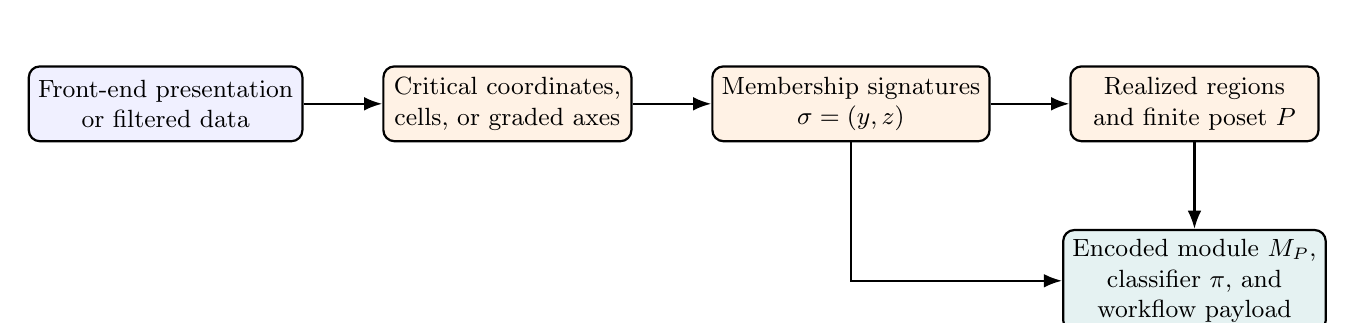
\begin{tikzpicture}[
		>=Latex,
		node distance=8mm and 10mm,
		every node/.style={font=\small},
		box/.style={rounded corners, draw, thick, align=center, minimum width=3.0cm, minimum height=0.95cm, fill=blue!6},
		midbox/.style={rounded corners, draw, thick, align=center, minimum width=3.15cm, minimum height=0.95cm, fill=orange!10},
		outbox/.style={rounded corners, draw, thick, align=center, minimum width=3.2cm, minimum height=1.05cm, fill=teal!10}
		]
		
		\node[box] (pres) {Front-end presentation \\ or filtered data};
		\node[midbox, right=of pres] (cells) {Critical coordinates, \\ cells, or graded axes};
		\node[midbox, right=of cells] (sig) {Membership signatures \\$\sigma=(y,z)$};
		\node[midbox, right=of sig] (poset) {Realized regions \\and finite poset $P$};
		\node[outbox, below=11mm of poset] (enc) {Encoded module $M_P$, \\classifier $\pi$, and \\workflow payload};
		
		\draw[->, thick] (pres) -- (cells);
		\draw[->, thick] (cells) -- (sig);
		\draw[->, thick] (sig) -- (poset);
		\draw[->, thick] (poset) -- (enc);
		\draw[->, thick] (sig.south) |- (enc.west);
		
	\end{tikzpicture}
	\caption{The common structure of the encoding algorithms.  The front end determines finitely many critical cells or grades; these are labeled by membership signatures; equal signatures are merged into regions; and the resulting finite region poset supports the encoded module and classifier map.}
	\label{fig:encoding-pipeline}
\end{figure}

\subsection{The finite-poset case}

The easiest encoding case is the one in which the input already lives on a finite poset.  If a module is already given as a finite-poset module or through a finite fringe presentation on a finite poset $P$, then there is no geometric compression left to perform.  One may simply take
\[
\pi = \mathrm{id}_P,
\qquad
H=M,
\]
and regard the given module as already encoded.

This seemingly trivial case is nevertheless architecturally important, as it fixes the target language for every other encoding routine.  The point of the nontrivial encoders is not to invent some new sort of output object, but to reduce back to this finite case.  This is why the user-facing workflow still packages a finite poset input into the same kind of result object used everywhere else, which is the \texttt{EncodingResult} object.

In practice, this finite case also provides the normalization point for correctness checks.  Whenever a more geometric encoder is tested, the resulting finite module is compared against the module obtained by evaluating the original front end presentation on the encoded regions.  Thus, the finite poset case is conceptually degenerate but mathematically definitive.

\subsection{Encoding flange presentations over $\mathbb{Z}^n$}
\label{subsec:encoding-zn}

We now come to the first actually nontrivial encoding algorithm.  Suppose the input is a flange presentation over $\Z^n$, as introduced in section~\ref{sec:pre-encoding}.  Concretely, we are given finitely many flats $F_1, \dots,F_m$, finitely many injectives $E_1, \dots,E_r$, and a matrix
\[
\Phi \in \kk^{r \times m}
\]
with the usual support condition.  The ambient poset $\Z^n$ is infinite, so the purpose of the encoder is to replace these data by a finite region poset.

The first observation is that the membership of a lattice point in a flat or injective can change only when one crosses one of finitely many coordinate thresholds.  Indeed, each flat and each injective is defined by finitely many affine coordinate inequalities, so along each coordinate axis there are only finitely many critical integers coming from the generator boundaries.  Collect these critical integers on axis $i$ into a sorted list
\[
c_{i,1}<c_{i,2}< \cdots<c_{i,k_i}.
\]
These values cut the lattice into rectangular slab cells.  A slab cell records, for each coordinate, whether the point lies before the first critical integer, exactly on a critical integer, or between consecutive critical integers.  Any two lattice points lying in the same slab cell have the same membership in every flat and every injective.  Hence the signature is constant on each slab cell.

The implementation reflects this observation through its representation of the classifier, a \texttt{ZnEncodingMap}, which stores:
\begin{itemize}[leftmargin=1.5em]
	\item the ambient dimension $n$;
	\item the critical-coordinate lists on each axis;
	\item the realized $y$- and $z$-signature rows;
	\item a representative lattice point for each encoded region;
	\item a dictionary from signatures to region indices;
	\item and, when available, a direct slab-cell-to-region lookup table.
\end{itemize}

The algorithm proceeds in four conceptual steps.

\smallskip
\textbf{Step 1: build the critical coordinate axes.}
From the flange generators one extracts the finitely many relevant coordinate thresholds.  These are stored axis by axis and determine the discrete slab decomposition.  The point of this step is not yet to decide which regions are nonempty or distinct, but only to identify a finite search space in which the signature can change.

\smallskip
\textbf{Step 2: evaluate realized signatures on slab representatives.}
Each slab cell admits a representative lattice point, and the code evaluates that representative against the flat and injective families.  The resulting signature is the pair
\[
\sigma(g)= \bigl(y(g),z(g) \bigr),
\qquad
y_i(g)=1 \iff g\in F_i,
\qquad
z_j(g)=1 \iff g \notin E_j.
\]
Cells with the same signature are merged.  In the implementation the signature rows are bit-packed, so that large families of generators can still be compared quickly and stored compactly.

\smallskip
\textbf{Step 3: form the finite region poset.}
The realized signatures are partially ordered by componentwise inclusion.  This yields the finite signature poset
\[
P= \{ \text{realized signatures}\},
\qquad
\sigma \leq \sigma' \iff \sigma \text{ is componentwise contained in } \sigma'.
\]
This is the finite encoding poset.  The classifier map
\[
\pi : \Z^n \to P
\]
sends a lattice point to the signature of the slab cell containing it.

\smallskip
\textbf{Step 4: push the presentation to the finite poset.}
The original flats and injectives are pushed forward to upsets and downsets in $P$.  The presentation matrix is then monomialized: entries that correspond to pairs of pushed-forward generator and relation regions that do not intersect are set to zero.  This enforces the same support condition on the encoded finite fringe presentation that the original flange satisfied in the lattice.

The output of this stage is therefore not just the finite poset $P$ but an actual finite fringe module on $P$, together with the classifier map and region representatives.  The workflow layer then materializes, when needed, the corresponding finite poset module.

There are also two important implementation consequences.

Firstly, point location becomes fast.  Once the slab-cell lookup table has been built, locating a lattice point means determining which slab cell it lies in and then reading off the region index.  This is one of the reasons the $\Z^n$ encoding route supports later invariant queries efficiently.

Secondly, encodings can be reused.  The code records an encoding profile determined by the ambient dimension and the underlying flat and injective families.  This allows later pushforward plans, region masks, and compiled lookup data to be cached and reused across repeated queries or across collections of modules that share the same geometric encoding problem but differ only in coefficients or in the presentation matrix.  This is especially important when several modules are encoded at once over the same poset.

Indeed, this simultaneous encoding case is built into the workflow.  When a finite collection of flanges is encoded together, the library first constructs a single common region poset $P$ and a single classifier map $\pi$, and only then pushes each flange to that common target.  This is essential for later comparison and bifunctorial constructions such as Hom and Ext, since those operations require their arguments to live on a common finite poset model.

\subsection{Encoding PL and box presentations over $\mathbb{R}^n$}
\label{subsec:encoding-rn}

The situation with real parameters is formally similar but geometrically richer.  A PL fringe presentation again consists of finitely many upsets, finitely many downsets, and a matrix relating them.  The encoding problem is to partition the relevant part of $\R^n$ into finitely many regions on which the signature is constant and then to pass to the corresponding finite poset.

In \TAMER{} this is implemented through two complementary back ends.

\subsubsection*{The box-specialized backend}

When the input consists of axis-aligned box upsets and box downsets, the encoding can be performed much more directly than in the general polyhedral case.  Along each axis one again extracts the finitely many coordinate values occurring as lower or upper bounds of the generators.  These values define a rectangular cell decomposition of the ambient space.  Every open or half-open cell in this decomposition has constant membership in every box generator, so signatures are constant on cells.

The implementation exploits this aggressively.  Rather than re-evaluating every generator independently on every cell representative, it traverses the cells in boustrophedon order and updates the signature incrementally.  Crossing a coordinate boundary can only affect the generators whose threshold is met at that boundary, so the signature update is sparse.  In this way, the full grid of cells is traversed once, realized signatures are deduplicated, and a direct cell-to-region lookup table is built.

This backend therefore has a very transparent geometry:
\begin{enumerate}[label=(\roman*)]
	\item collect coordinate thresholds;
	\item build the rectangular cell grid;
	\item traverse cells and compute signatures;
	\item merge equal signatures into regions;
	\item order the regions by componentwise signature inclusion;
	\item push the original presentation to the resulting finite poset.
\end{enumerate}

The output classifier is a \texttt{PLEncodingMapBoxes}.  Besides the region signatures and representatives, it stores the coordinate axes, the mixed-radix cell shape and strides, and a cell-to-region table.  As in the lattice case, this supports fast repeated point location.  In particular, when a point lies away from a cell boundary, location is a direct mixed-radix lookup.

\subsubsection*{The general PL/polyhedral backend}

Axis-aligned boxes occur often enough that they merit their own specialized backend, but they are not the only natural real parameter front end.  In many situations the relevant generators and cogenerators are fully polyhedral: they are cut out by arbitrary linear inequalities and therefore meet along oblique facets rather than along coordinate hyperplanes.  The ambient parameter space is then divided by a finite collection of polyhedral boundaries, and the resulting constant regions of the module need no longer be rectangular.  The general PL backend is designed for exactly this richer setting.

The first implementation decision is to represent each convex piece by an explicit halfspace description
\[
A x \leq b
\]
stored over the exact coefficient field \( \Q \).  This is important because the encoder needs an exact description of the geometry while it is deciding which signatures are actually realized, and floating-point approximations may be too inexact. 

Additionally, we plan our algorithm so that point membership tests do not depend on a particular version of an external polyhedral package in \texttt{Julia}, like \texttt{Polyhedra} or \texttt{CDDLib}. So, the basic polyhedral object stores the \(H\)-representation itself, and membership in a convex piece or a finite union of such pieces is evaluated directly from the stored inequalities.

This leads to the second design decision, which is to avoid building the full polyhedral arrangement explicitly.  In principle one could intersect every boundary hyperplane with every other and attempt to construct the full cell decomposition of the arrangement.  In practice that would be the wrong primitive: the arrangement remembers far more geometry than the module itself uses, and its combinatorial complexity can be much larger than the number of distinct module regions.  The backend therefore prioritizes signatures rather than arrangements.

Suppose the input presentation is
\[
\varphi \colon \bigoplus_{i=1}^{m} \kk\{U_i\}
\longrightarrow
\bigoplus_{j=1}^{r} \kk\{D_j\},
\]
where each \(U_i\) is a PL upset and each \(D_j\) is a PL downset, each given as a finite union of convex polyhedra.  As in the earlier discussion of signatures, one seeks the pairs
\[
(y,z) \in \{0,1\}^{m} \times \{0,1\}^{r}
\]
that are actually realized by points of \(\R^n\), where \(y_i\) records membership in \(U_i\) and \(z_j\) records non-membership in \(D_j\).  The naive search space is still finite, but potentially large, so the implementation is organized around a branch feasibility strategy that only keeps signatures that are geometrically realizable, which we will now describe.

The central observation is that membership in a finite union is a disjunction over its convex pieces, while non-membership is the conjunction of being outside every piece.  The encoder resolves those two logical forms differently.

If a signature requires a point to lie inside a PL upset or downset, the algorithm chooses one convex piece from that union and adds its full \(H\)-representation to the running system.  If a signature requires a point to lie outside a PL upset or downset, the algorithm does not try to complement the whole polyhedron directly.  Instead, for each convex piece it chooses one facet inequality to violate.  Thus ``outside a union'' becomes a finite family of exact feasibility branches, each one encoded by selecting, for every relevant piece, a single facet that must be crossed.  Internally, these outside conditions are implemented as strict violations
\[
a^\top x > b
\]
which are converted into exact closed inequalities
\[
a^\top x \geq b + \varepsilon
\]
for a fixed rational slack \(\varepsilon > 0\).  In this way, strictness is handled symbolically rather than numerically.  Once the chosen ``inside'' and ``outside'' conditions have been assembled, the backend builds a single exact polyhedron from the combined inequalities and asks whether it is empty.  If it is nonempty, the signature is realized; if it is empty, the branch is discarded.

This procedure is encapsulated in the feasibility enumeration routine.  Its output is not the whole arrangement, but a list of realized signatures together with a polyhedral representative for the corresponding region and, when available, a witness point extracted from a \(V\)-representation.  The witness is not logically necessary for correctness, but it is extremely useful later: it gives the backend a cheap representative point for region-level queries, candidate ordering in point location, and later geometric summaries.  

The enumeration routine also collapses repeated signatures.  Distinct feasibility branches can describe different polyhedral pieces of the same signature class, but from the point of view of the encoded module those pieces are equivalent.  It is therefore the signature, not the raw region geometry, that determines the finite encoding poset.

Once the realized signatures have been collected, the backend constructs the finite region poset.  There are two closely related choices.  In the first, the realized signatures themselves are ordered componentwise, producing the signature poset.  In the second, one passes to a denser uptight refinement derived from the same signatures.  The user-facing choice is recorded through the option \texttt{poset\_kind}.  In either case the result is a finite poset \(P\) whose vertices correspond to module regions rather than to geometric cells of the ambient arrangement.

The original PL presentation is then pushed down to \(P\).  For each original upset generator \(U_i\), one forms its image on \(P\) by marking precisely those realized signatures in which the \(i\)th \(y\)-bit is active; dually, for each downset generator \(D_j\), one marks those realized signatures in which the \(j\)th \(z\)-bit is inactive.  These masks are closed upward or downward inside the finite poset to obtain honest upsets and downsets on \(P\).  The coefficient matrix is then monomialized: if the pushed-forward upset and downset corresponding to an entry \(\Phi_{ji}\) are disjoint in the finite region poset, that entry is set to zero.

The output of the backend is therefore a triple
\[
(P,H,\pi),
\]
where \(P\) is the finite region poset, \(H\) is the pushed-down finite fringe module on \(P\), and \(\pi\) is a classifier from \(\R^n\) to \(P\).  The classifier is represented by a \texttt{PLEncodingMap}, which stores not only the signature data and region representatives, but also a compiled collection of fast geometric surrogates used for repeated point queries.

This compiled point location layer is one of the main practical devices that makes this backend usable.  Exact polyhedral feasibility is too expensive to rerun every time an invariant routine asks where a point lies.  The encoder therefore precomputes floating-point copies of the halfspace systems for each region, in both strict and slightly relaxed forms.  These do not replace the exact geometry used during encoding, but they provide a fast and robust numerical filter for later queries.  Given a point \(x\), the classifier tests candidate regions by evaluating the stored float halfspaces with a controlled tolerance.  Because the regions are already known to be exact from the encoding stage, this floating-point layer is a search mechanism rather than a source of mathematical ambiguity.

The candidate set itself is reduced by several prefilters.  The simplest uses witness points: regions are partially ordered according to one witness coordinate, and a query need only inspect a short window around the corresponding coordinate of the query point.  When the ambient dimension is at least three and the witness cloud has informative variance in several coordinates, the backend builds a multi-projection prefilter that keeps a small candidate family consistent across several projected orderings at once.  In dimensions one and two, when enough regions are present and exact region bounding boxes can be obtained, the backend also builds a coarse spatial bucket index from region bounding boxes.  This allows a query point to be routed immediately to a small list of nearby candidate regions.  The net effect is that point location is usually much cheaper than a full scan of all polyhedral regions, even though the exact encoded geometry may be complicated.

The same philosophy appears in the batched query routines.  If a large matrix of query points is supplied, the backend groups points by bucket and applies the same candidate sets repeatedly, with threading heuristics that switch on only when the expected work is large enough.  In other words, the PL backend is not only exact at construction time; it is also engineered for repeated evaluation after construction.  That matters because many later invariants, especially slice-based and geometric ones, call the classifier many times.

The general PL backend is also the route by which the library supports common encoding of several PL fringe presentations at once.  In that case the upsets and downsets from all inputs are pooled, feasibility enumeration is performed once on the combined family, and the resulting common region poset is then sliced back into one pushed down fringe presentation for each input module.  This is a substantial advantage of the general backend over the box-specialized route: once several modules have been encoded into the same finite poset, later comparisons such as Hom, Ext, and distances can be carried out directly on a common finite model.  

\subsection{Geometry attached to an encoding map}
\label{subsec:encoding-geometry}

Having now reviewed how each front end type is treated through encoding, we now consider the geometry obtained with that encoding. The encoding step produces more than just a finite poset and a classifier.  Indeed, it also produces a finite stratification of the ambient parameter space.  Once this stratification exists, one may ask geometric questions about its regions.

At the most basic level, every encoding provides region representatives and, when possible, axes derived from the encoding.  In grid-like settings these axes are simply the critical coordinates together with representative values for the intervening slabs.  More refined questions are backend-sensitive.  For a region one may ask for a bounding box, coordinate widths, a centroid, a diameter, or a measure of its boundary.  For a whole encoding one may ask which regions are adjacent, how large the interfaces between them are, or how much volume each region occupies inside a chosen window of the ambient parameter space.

This geometric layer is not another pre-encoding input type.  That is, the regions whose geometry is being measured are not the original front-end generators, but the strata produced by the encoding itself.  In other words, region geometry is an attribute of the encoded decomposition of parameter space, not of the initial presentation data.

\subsection{From filtered data to finite encodings}
\label{subsec:data-to-encoding}

The front ends discussed so far begin with explicit presentations. But, the data ingestion step occurs earlier, with filtered data.  Its task is to convert raw data into a finite algebraic object that can be encoded by the same workflow.

There are two main internal representations at this stage: labeled cell complexes and packed simplex trees.

A labeled cell complex records cells, boundary matrices, and the multigrade of each cell.  This is the correct representation for a general finite filtered cell complex.  A \texttt{SimplexTreeMulti} records the same sort of information for simplicial data in a more compressed form.  Concretely, it stores the vertices of all simplices in flattened arrays together with offset tables, simplex dimensions, and the grade data attached to each simplex.  The point of this packed representation is that one can traverse simplices and grades without first expanding the full boundary structure into a dense or redundant intermediate object.

The filtration family, for example a Rips-type, lowerstar, graph-type, cubical, or Delaunay-type filtration, assigns grades to the combinatorial pieces of the raw dataset.  The result is either a labeled cell complex directly or, when the route is simplicial and compactly representable, a simplex-tree object together with the same essential grading information.

The encoding step for such objects differs from the fringe and flange cases in in that here the front end object is already finite.  The issue is not that the indexing poset is infinite, but that the labeled cell complex is not yet organized as a reusable finite poset module.  The ingestion layer therefore turns the finite set of occurring grades into axes, forms the corresponding grid or product-of-chains poset, and then computes the appropriate cochain or cohomology object on that finite poset.

More concretely, the ingestion workflow performs the following steps.
\begin{enumerate}[label=(\roman*)]
	\item Starting from the raw data and filtration specification, build a labeled cell complex or a simplex tree.
	\item Extract the finite coordinate axes determined by the grades.  Optional quantization, axis policies, and coarsening may be applied at this stage.
	\item Build the finite grid poset $P$ determined by those axes and by the chosen orientation convention.
	\item Construct a cochain complex over $P$, either lazily from the packed simplex tree or directly from the labeled cell complex.
	\item Compute the requested output stage: a cochain complex, a module, a fringe presentation, a flange (in the integer-axis case), cohomology dimensions, or a full \texttt{EncodingResult}.
\end{enumerate}

Thus, the endpoint is the same as for the presentation-based encoders, the \texttt{EncodingResult}.  Once the cohomology module on the finite grid poset has been built, it is packaged as an encoded object with a classifier map.

\subsection{Common encodings}

Many later computations involve more than one module.  Hom, Ext, interleaving-style comparisons, common feature extraction, and benchmarking against shared inputs all require the objects being compared to be represented against a common finite combinatorial model whenever possible.  For this reason the encoding layer supports common encodings.

In the lattice case, several flange presentations can be encoded simultaneously by constructing a single common signature poset and a single classifier map, then pushing each presentation to that common target.  In the real case, common encoding is supported for collections of compatible PL inputs, with some backend specific restrictions.  If modules are already finite poset modules on different finite posets, the library also supports comparison by passing to a common refinement, typically a product poset.

\section{Post-encoding algebra on finite posets}\label{sec:post-encoding-algebra}

Once the encoding step has been completed, the diverse front ends described in the previous chapters have all been converted into the same kind of object: a module on a finite poset together with the classifier map that relates that finite object to the original parameter space.  This is the point at which the library's mathematical scope changes.  Before encoding, the central issue is how to represent geometric or combinatorial input data by finite descriptions.  After encoding, the central issue is what one can do with a finite poset module once one has it.

The main point is not merely that finite encodings make later computations faster, although they do.  The deeper idea is that a finite encoded module supports a much richer range of exact algebraic constructions than any summary invariant can.  Instead of discarding the module after extracting ranks, slice barcodes, or images, \TAMER{} retains an algebraic object and performs category theory and homological operations on that object.  In particular, the codebase supports not only direct constructions such as kernels, cokernels, Hom, Ext, and Tor, but also more structured objects such as projective and injective resolutions, mapping cones, distinguished triangles, RHom complexes, derived tensor products, hyper-Ext and hyper-Tor spaces, and transport functors along maps of finite posets.

The mathematical foundation for doing this is entirely classical: for a finite poset $P$, the category of $P$-modules is an abelian category, and many standard constructions can be expressed explicitly in finite-dimensional linear algebra \cite{Mac98,Wei94}.  What is new in the present context is that the library chooses finite-poset modules as its working language after encoding, so these classical constructions become part of the ordinary computational workflow rather than remaining only in the formal background.  This is also where Miller's tame module perspective becomes especially concrete: once a module has been encoded by a finite poset, one may carry out constructions that the syzygy theorem predicts should exist \cite{Mil20}.

\subsection{Encoded modules and morphisms as the internal working language}

The internal algebraic language of the library is the category of modules over a finite poset.  If $P$ is a finite poset, a $P$-module is a functor
\[
M : P \longrightarrow \mathbf{Vect}_{\kk},
\]
and a morphism $f\colon M\to N$ is a natural transformation.  In the implementation these are represented by the types \texttt{PModule} and \texttt{PMorphism}.  The key design choice is that, once an input has been encoded, all subsequent exact algebra is phrased in terms of these finite poset objects, regardless of whether the module originally came from a flange, a PL fringe, or filtered data.

At a purely formal level, one could store every structure map
\[
M(p\leq q) : M(p)\to M(q)
\]
for every comparable pair $p \leq q$ in $P$; that would be correct but wasteful.  The code instead stores the module along cover edges and reconstructs longer comparable maps on demand by composition.  This is possible because the partial order is finite, and because the functoriality relations force every longer map to be the composite of cover edge maps.  In practice this matters a great deal.  The finite poset layer maintains cover edge data structures and cached query mechanisms for repeated requests of the form ``what is the map from $p$ to $q$?''  The user-facing routine \texttt{map\_leq} computes a single such map, while the batched routines \texttt{map\_leq\_many} and \texttt{prepare\_map\_leq\_batch} reduce repeated transport along comparable pairs to a cached composition problem.

This design explains why encoded modules are practical even when the ambient input geometry was complicated.  Once the module has been pushed to a finite poset, the data to be stored are finite, and the recurring structural questions are reduced to finite matrix calculations.  It also explains why the post-encoding part of the library insists on full module objects rather than only on dimension tables or rank summaries. Mainly, a dimension table cannot answer a map query, but a finite-poset module can.

The workflow layer makes this internal language visible to the user without forcing the user to build these objects manually.  An \texttt{EncodingResult} stores a finite poset $P$, an encoded module $M$ on $P$, a classifier map $\pi$, and, when available, pushed-down presentation data.  The downstream algebraic routines work with the encoded module itself.  If two encoded modules live on the same finite poset, then they can be compared immediately.  If they do not, then the library either common-encodes them earlier in the workflow or constructs an explicit common refinement later, as discussed below.

\subsection{Abelian-category constructions in code}

Because $P$-modules form an abelian category, all of the familiar exact constructions are available. In the codebase, the \texttt{AbelianCategories} layer implements kernels, images, cokernels, coimages, quotients, submodules, pushouts, pullbacks, biproducts, products, coproducts, equalizers, coequalizers, and more general limits and colimits.  It also packages short exact sequences as explicit checked objects and includes a computational version of the snake lemma.

The importance of these constructions is easiest to see from ordinary persistence questions.  Suppose one has a comparison map between two encoded modules coming from two nearby filtrations.  The image of that map records what is shared by the two modules, while the kernel and cokernel record the discrepancy.  If one has two maps with a common codomain, the pullback computes the fiber product object on which the two induced maps agree; dually, a pushout combines two modules along a common submodule. If one is studying a sequence of models that is supposed to be exact, the library can package that claim as a \texttt{ShortExactSequence} and verify it pointwise and naturally.

In multiparameter persistence, many constructions that are easy to state geometrically are most naturally analyzed via such exact algebra.  One may want, for example, the image of a map induced by changing a filtration, the pullback of two competing comparison maps, or the connecting morphism produced by the snake lemma.  A system focused on summaries first would have to rebuild these indirectly from invariant data, if that were possible at all. In contrast, once the encoded module category is present explicitly, these are first class computational objects in \TAMER.

The snake lemma is an especially telling example.  In the codebase it does not just assert the existence of a connecting homomorphism: it returns all six modules and five maps in the resulting exact sequence as actual morphisms of finite poset modules.  That illustrates the general philosophy of the post-encoding stage.  The implementation is not satisfied with knowing that a construction exists abstractly.  It attempts, whenever feasible, to return the construction itself in the same internal algebraic language.

\subsection{Indicator resolutions, projective covers, and injective hulls}

The next layer of structure regards resolution theory.  Section~\ref{sec:tameness} explained that one of the main manifestations of tameness is the existence of finite presentations and resolutions by indicator modules.  After encoding, this becomes concrete.  The finite poset module category contains explicit analogs of projective and injective building blocks, namely principal upset and principal downset modules.  In the codebase these are assembled through the \texttt{IndicatorResolutions} layer.

Given an encoded module $M$ on a finite poset $P$, the library can compute a projective cover of $M$ and an injective hull of $M$.  From there it can build successive upset resolutions and downset resolutions.  The routines \texttt{projective\_cover}, \texttt{injective\_hull}, \texttt{upset\_resolution}, \texttt{downset\_resolution}, and \texttt{indicator\_resolutions} make these constructions explicit.  The corresponding verification routines check exactness and connectedness conditions in the resulting indicator complexes.

This is the moment when Miller's syzygy theorem becomes algorithmic.  The theorem says that finite encoding, finite fringe presentation, and finite indicator resolutions are equivalent viewpoints on tameness \cite{Mil20}.  The implementation uses that equivalence in the forward direction: once a module has been finitely encoded, the library can dominate that encoding by explicit upset and downset resolutions, just as the theorem predicts.

These constructions are useful for at least three different reasons.  Firstly, they are the input to derived functor computations.  Secondly, they provide algebraic summaries in their own right, such as Betti and Bass multiplicities on the encoding poset.  Thirdly, they expose how the module is assembled from order theoretic pieces of the poset.  That last point is especially valuable in a persistence setting, because the principal upsets and downsets play a role analogous to births and deaths, but in a language that continues to make sense even when no barcode classification exists.

One should, however, be careful about minimality.  In the general theory over arbitrary posets, minimality is subtle \cite{Mil20}.  The codebase therefore treats minimality as a diagnostic and certification problem. For projective and injective resolutions on finite encoded modules, the library provides minimality reports and checked constructions of minimal Betti and Bass summaries when the relevant assumptions are satisfied.

\subsection{Derived functors and structure for complexes}

The most distinctive consequence of retaining an encoded finite poset module is that one can perform nontrivial homological algebra directly.  The \texttt{Workflow} and \texttt{DerivedFunctors} layers expose the most familiar constructions first: \texttt{hom}, \texttt{ext}, and \texttt{tor}.  If two encoded modules lie on the same finite poset, \texttt{hom} computes the internal Hom space of natural transformations between them, and \texttt{hom\_dimension} provides a fast dimension-only route when a basis is not needed.  The routine \texttt{ext} computes higher Ext groups using either projective or injective models, while \texttt{resolve} constructs the chosen resolution together with Betti or Bass information.

The Tor calculation requires a mild but important hypothesis.  Since Tor couples a right module with a left module, the first argument must be represented as a module on the opposite poset.  In the workflow layer this is made explicit: if one asks for
\[
\operatorname{Tor}(R^{\mathrm{op}},L),
\]
then the encoded module corresponding to $R^{\mathrm{op}}$ must live on the opposite finite poset of the one on which $L$ lives.  The code supports two computational models, depending on which side is resolved, but the opposite poset requirement is not optional. However, because the poset is finite and represented concretely, its opposite can be formed and checked directly.

The scope of the implementation goes beyond these first derived functors.  The library also supports an Ext algebra with Yoneda product, functorial maps in either variable, long exact sequences, and various comparison morphisms between different resolution models. At the chain-complex level, the \texttt{ModuleComplexes} and \texttt{ChainComplexes} layers provide module cochain complexes, cochain maps, cochain homotopies, mapping cones, distinguished triangles, quasi-isomorphism tests, and explicit cohomology modules.  On top of those, one has RHom complexes, derived tensor complexes, hyperExt spaces, and hyperTor spaces, together with maps induced in the first or second variable.

The same is true of spectral sequence constructions.  The codebase includes double complexes, total complexes, spectral sequences, and helper routines for page data, filtrations, edge maps, and convergence reports.


\subsection{Change of posets, transport, and comparison}

Finite encoding also makes it natural to transport modules along explicit maps of posets.  This is handled by the \texttt{ChangeOfPosets} layer.  If $\pi : Q\to P$ is a monotone map between finite posets, the library supports pullback or restriction along $\pi$, left and right pushforwards along $\pi$, and their derived versions.  In categorical language these are Kan extension constructions; computationally they are implemented by exact finite linear algebra on the fibers of the map.

These transport operations are essential for comparison.  If two modules are already encoded on the same finite poset, then comparison is immediate.  If not, one may still compare them by constructing a common refinement.  The library includes routines for encoding a family of finite poset modules into a common refinement poset.  This matters because many algebraic operations, including Hom and Ext, require the inputs to live on the same underlying poset object.  The transport layer therefore serves as the bridge between the geometric fact that two modules originate from different parameterizations and the algebraic requirement that they be brought into a common finite context before exact comparison can begin.

The interaction between transport and derived functors is particularly fruitful.  Because encoding maps are explicit, one can pull back and push forward not only modules but also morphisms, resolutions, and complexes.

\subsection{What computational opportunities this opens}

The post-encoding algebraic layer changes what kinds of computational questions can even be asked.  The contrast with summary-first multiparameter software is therefore not merely that \TAMER{} exposes more functions in an interface.  The deeper difference is representational: because the encoded output is an algebraically expressive finite object, the library can support workflows that would otherwise be inaccessible.

One family of such workflows concerns naturality and comparison.  Given two filtrations and a comparison map between them, one can encode the resulting modules, compute the induced morphism, and then study its kernel, image, cokernel, or mapping cone.  Another family concerns resolution-based information.  Instead of stopping once the module has been encoded, one can compute projective and injective approximations, Betti and Bass data, or Ext and Tor spaces, or convolutions arising from the sheaf theory perspective \cite{KS18}.  Yet another family concerns transport.  When modules naturally live on related but different finite posets, one can move them along explicit poset maps or refine them to a common comparison setting.  All of these are ordinary algebraic activities once the encoded module exists; none of them is naturally expressible if one has already replaced the module by a rank table, a set of slices, or an image.

This is, again, the key reason the explicit encoding architecture matters scientifically.  In one-parameter persistence, the barcode is often enough because it already carries a very large fraction of the interesting structure.  In several parameters, that is no longer true.  The right response is not to abandon invariants, but to delay the choice of invariant until after one has built a finite algebraic model rich enough to support many of them.  The next chapter follows that logic directly: once the encoded finite-poset module has been constructed and placed in its algebraic context, one can ask what summaries and invariants are best extracted from it for interpretation, statistics, and downstream applications.

\section{Invariants and summaries after encoding}\label{sec:invariants}

The encoded finite-poset module is the primary output of the library, but it is not usually the final object one wishes to inspect.  In applications one typically wants a summary, a comparison value, a visual object, or a fixed size descriptor that can be exported to a downstream pipeline.  The main lesson of multiparameter persistence is that no single such invariant can play the role of the ordinary barcode.  Different invariants retain different parts of the structure, and they are useful for different reasons.  The right question is therefore not how to force all information into one descriptor, but which part of the encoded module one wants to emphasize for the task at hand.

This is exactly how the invariant layer of \TAMER{} is organized.  Every invariant in this chapter is computed from the same encoded object, usually an \texttt{EncodingResult} carrying a finite poset module $M$ and classifier map $\pi$.  Some invariants are exact algebraic functions on the encoded module, such as dimensions or ranks of structure maps.  Some are built by restricting to one-parameter slices and then applying one parameter constructions.  Some combine the encoded algebra with the geometry of the regions produced by the PL backends.  Some convert cumulative data into sparse signed measures by Mobius inversion.  Others produce fixed-size images or tensor-valued summaries for statistical workflows.  What unifies them is not a common output type, but the fact that they all factor through the finite encoding.

We will now provide an overview of the invariant families implemented, without listing out actual functions or implementation details -- these can be perused instead in the code documentation or the reference material, respectively.

\subsection{Restricted Hilbert and rank-type invariants}

The simplest post-encoding summaries are the ones that read the finite poset module directly.  If $M$ is a module on a finite encoding poset $P$, its restricted Hilbert function is the dimension function
\[
h_M(p)=\dim_{\kk} M(p),\qquad p\in P.
\]
This is the most immediate size invariant of the encoded module.  It forgets all structure maps, but it records where the module is large, where it vanishes, and how its dimension varies across the encoding poset. The output is a finite vector or array indexed by the vertices of the encoding poset, so it is already suitable for plotting, thresholding, or later Mobius inversion.

A richer but still direct family is obtained by inspecting the structure maps themselves.  For comparable elements $a\leq b$ in the encoding poset, one defines the rank map
\[
\rho_M(a,b)=\operatorname{rank}\bigl(M(a\leq b)\bigr).
\]
Taken over all comparable pairs, this gives the rank invariant of the encoded module.  In one parameter persistence the rank invariant is equivalent to the barcode under the standard finiteness hypotheses, but in several parameters it is only one invariant among many \cite{CZ09,Les15}.  Nevertheless, it remains extremely important because it is exact, computable on the finite encoding, and closely tied to both slice-based and signed-measure constructions.

What is gained by studying this family is precision.  Restricted Hilbert data and rank data are the least mediated summaries in the whole invariant layer.  They retain exact information about the encoded module itself rather than about a secondary geometric surrogate.  For that reason they are often the right tools when one wants to compare modules algebraically, identify loci of constancy or jump, or build later invariants by inversion.

\subsection{Slice-based invariants and distances}

A second family of invariants is obtained by restricting a multiparameter module to one parameter slices.  If $\lambda : Q'\to P$ is a monotone map from a totally ordered set or chain into the finite encoding poset, then the pullback
\[
\lambda^*M=M\circ \lambda
\]
is an ordinary one parameter persistence module.  One may therefore compute its barcode and any one parameter summary derived from that barcode.  In practice, the slices of greatest interest are affine lines of positive slope in two parameters or monotone chains in a finite grid. Conceptually, the output is a family of ordinary persistence barcodes indexed by the chosen slice parameters.

This family matters because it is the main bridge between multiparameter and one parameter persistence.  It allows the user to view a complicated encoded module through a collection of one dimensional probes, each of which can be analyzed by familiar methods.  This is the idea behind fibered barcodes and interactive slice tools such as RIVET \cite{LW15}.  It is also the basis of the matching distance, which compares two modules by taking the supremum of weighted bottleneck distances over an appropriate family of slices.  The matching distance viewpoint originates in multidimensional size theory and persistent Betti numbers \cite{BCFGL08}, while exact polynomial-time computation in the biparameter case is due to Kerber, Lesnick, and Oudot \cite{KLO20}.

The same section of the codebase also supports a more sheaf-theoretic projection philosophy.  Projected barcodes and projected distances treat one parameter shadows of a multiparameter module as derived pushforwards to $\R$, rather than only as literal restrictions to affine lines \cite{BP24}.  The corresponding implementation builds projected arrangements and projected-barcode caches, and then computes scalar projected distances or kernels from those objects.  These outputs are not barcodes in the usual sense, but finite families of one parameter descriptors obtained from the encoded module by a controlled transport construction.

The gain here is flexibility.  Slice invariants are, of course, not complete, but they are often interpretable, stable, and far more tractable than global comparison invariants such as interleaving distance.  They are also naturally suited to caching: once the encoded module has been equipped with projected or fibered slice plans, many repeated slice queries can be answered cheaply.

\subsection{Geometry of encoding regions and weighted summaries}

Some post-encoding summaries are not purely algebraic functions of the finite poset module.  They also depend on the geometry of the encoding regions.  This is especially important when the encoding arose from the PL or box backends, because in that setting the classifier map identifies actual regions in parameter space.  Those regions come with geometric information such as volume, bounding boxes, widths, diameters, aspect ratios, boundary measures, and adjacency relations.  Section~\ref{subsec:encoding-geometry} introduced this geometry as part of the encoding layer.  Here it becomes a source of invariants.

The most basic use of region geometry is weighting.  If an algebraic quantity is constant on each encoded region, then one can integrate it back over the ambient parameter domain by weighting the regions appropriately.  This yields invariants such as support measure, integrated Hilbert mass, and the aggregate measure carried by a prescribed algebraic value.  In code, the outputs are generally scalar summaries, histograms, or dictionaries keyed by dimensions or value strata.

A second use of region geometry is shape and interface analysis.  Once region adjacency and boundary measure are available, one can study how algebraically distinct regions fit together in parameter space.  The code therefore includes summaries such as boundary-to-volume ratios, aspect-ratio statistics, adjacency-graph statistics.  The role of these constructions is to measure how the algebraic behavior of the module is distributed geometrically.  In particular, they allow one to distinguish between modules with similar combinatorial support but very different ambient geometry.  This is something that would simply be invisible in a purely rank- or slice-based summary.

\subsection{Mobius inversions, signed measures, and Euler-type summaries}

A recurring idea in the invariant layer is that cumulative information on a finite grid can often be inverted into a sparse local measure.  The basic mechanism is Mobius inversion on a finite product-of-chains poset.  This appears in several forms in the library.

The first is the rectangle signed barcode, also called the signed rectangle measure.  Starting from encoded rank data, one can write the rank invariant as an integer linear combination of rectangle or segment indicator contributions.  The general idea goes back to generalized persistence diagram constructions and their positivity properties \cite{Pat18}; for multiparameter rank decompositions and signed barcodes in the present sense, the relevant reference is the work of Botnan, Oppermann, and Oudot \cite{BOO22}.  In code, the output is a sparse signed collection of rectangles together with integer weights.  This object is more compact than the full rank table, can be visualized directly, and can be converted back into rank data on demand.

The second family is built from Euler data.  If one has a module cochain complex $C^\bullet$ on the encoding poset, then one may define the Euler surface by
\[
\chi_C(p)=\sum_i (-1)^i \dim_{\kk} C^i(p)
\]
on a chosen finite grid or set of axes.  In multiparameter settings, Euler surfaces and Euler profiles have been studied as computationally cheap topological summaries \cite{Bel22,DG23}.

The gain from these signed-measure families is compactness together with transportability.  A dense rank or Euler table can be large and awkward to compare directly.  A sparse signed measure records the same data in a local form, and it can then be turned into a kernel, an image, or a low dimensional feature vector.  In other words, Mobius inversion is one of the main mechanisms by which the library converts exact finite algebra into compact summaries without leaving the encoded setting.

\subsection{Multiparameter landscapes, persistence images, and image-like summaries}

The next family consists of invariants that represent the encoded module by sampled functions or raster images. At the one parameter level, the best known examples are persistence landscapes and persistence images. Persistence landscapes were introduced by Bubenik as stable function-valued summaries lying in a Banach space \cite{Bub15}.  Persistence images were introduced by Adams, Emerson, Kirby, Neville, Peterson, Shipman, Chepushtanova, Hanson, Motta, and Ziegelmeier as stable finite dimensional vectorizations of persistence diagrams \cite{AEK17}.  In the multiparameter setting, there are two natural generalizations in the codebase.

The first is slice aggregation.  One computes ordinary one parameter landscapes, images, silhouettes, entropies, or barcode summaries on a family of slices, and then aggregates them.  The implemented function returns a sampled tensor indexed by slice parameters and by the usual one parameter landscape coordinates.  This family should be understood as a structured collection of one parameter summaries glued together through the finite encoding.  Multiparameter persistence landscapes in the stronger functional sense were introduced by Vipond \cite{Vip20}, and that paper is the right conceptual reference for why such landscapes are stable and why they represent rank information in a form suitable for statistics.

The second is the multiparameter persistence image family. Here the code passes through an intermediate decomposition object, \texttt{MPPDecomposition}, and then rasterizes the result into an \texttt{MPPImage}.  The guiding reference is the work of Carriere and Blumberg on multiparameter persistence images \cite{CB20}.  In the implementation, the output is a fixed size raster image together with the axes and smoothing parameters used to create it.  This is especially useful in data analysis settings because it turns the encoded module into a finite numerical array that can be fed directly into standard statistical or machine-learning tools.  The corresponding kernels and distances live at the same level: they compare the resulting sampled objects, not the original module directly.

\subsection{Algebraic support descriptors}

A final family sits closer to combinatorial commutative algebra.  These invariants study where the encoded module, or its resolution theory data, is supported and how that support is stratified.  The central references here are the multigraded commutative-algebra viewpoint of Carlsson and Zomorodian \cite{CZ09}, the general background on multigraded algebra in Eisenbud and in Miller--Sturmfels \cite{Eis95,MS05}, and the persistence-specific support theory work of Harrington, Otter, Schenck, and Tillmann \cite{HOST19}.

In the library this family includes associated primes, minimal primes, socles, and weighted support summaries derived from Betti and Bass data.  Notably, the routines for Betti support measures and Bass support measures combine the support of homological data with region geometry, thereby giving a finite weighted description of where generators, relations, or co-relations are concentrated in parameter space.

This family is useful because it addresses questions that rank and slice invariants do not.  Rank data describes transport between fibers; support theoretic data describes where the module or its derived algebra lives.  In the multiparameter setting that distinction is often essential.  A module may have the same coarse dimension profile as another while differing dramatically in how its support decomposes into algebraically meaningful strata.  The support descriptor family therefore provides a more commutative algebra view of the encoded object, and it is one of the features that most clearly distinguishes an encoding-centered system from one based only on topological summaries.

\subsection{Why the invariant layer is organized this way}

The invariant layer is therefore deliberately plural.  Restricted Hilbert and rank-type invariants are exact and algebraic.  Slice-based invariants trade completeness for interpretability and tractability.  Geometry-weighted summaries reconnect the encoded module to the ambient parameter domain.  Signed measures and Euler surfaces compress cumulative data into sparse local objects.  Landscapes and persistence images provide fixed-size descriptors for statistics and learning.  Support-theoretic invariants bring in a commutative-algebraic view of the module's structure.

No one of these families captures everything; the encoded module remains the primary object.  The point of the invariant layer is that, once the finite encoding has been built, one can choose the right summary for the right question without rebuilding the entire computation from scratch.  The next section turns to the cross-cutting layers that make this workflow usable in practice: serialization, featurization, and visualization.

\section{Featurization, serialization, visualization, and introspection}\label{sec:cross-cutting}

The encoded module is also the point at which \TAMER{} becomes useful as a practical software system rather than only an algebraic engine.  Once an encoding has been built, users may want to export it, turn it into a fixed size numerical representation, inspect or visualize it in a notebook, and understand what an intermediate object actually contains without reading raw fields.  For that reason the library includes three cross-cutting subsystems (featurization, serialization, and visualization) together with a shared introspection layer for user-facing objects.

Featurization treats an encoded module as input to a typed feature plan.  Instead of asking users to assemble feature matrices by hand, the library provides typed featurizer specifications for restricted Hilbert data, Euler surfaces, slice and barcode summaries, signed-measure summaries, multiparameter landscapes and persistence images, Betti and Bass tables, and support-measure summaries.  Applying such a specification to a collection of samples returns a \texttt{FeatureSet}, which is a numerical matrix together with feature names, sample identifiers, and metadata describing how the features were produced.  At a larger scale, an \texttt{ExperimentSpec} packages several featurizers together with batching, cache, and output policy so that the same collection of encoded objects can be processed repeatedly and reproducibly.

Serialization addresses reproducibility and exchange.  The library can save and load datasets, pipeline specifications, encodings, fringe-like source objects, and expensive derived artifacts such as multiparameter image data.  The design is intentionally strict, where owned JSON formats are versioned and validated, while external adapters are kept separate from the internal storage contracts.  Just as important, the JSON layer does not force loading immediately.  A file can first be queried by \texttt{inspect\_json}, which returns a typed summary containing artifact kind, schema version, field, poset type, profile hints, and file size; only afterwards can one call the relevant \texttt{load\_*\_json} routine.  This discipline makes it practical to manage large collections of artifacts without relying on ad hoc filename conventions or hand inspection of raw JSON.

Visualization is treated similarly.  Rather than tying mathematical objects directly to a single plotting backend, the library first builds inspectable \texttt{VisualizationSpec} objects.  A user can ask \texttt{available\_visuals(obj)} to see which views are supported, call \texttt{visual\_spec(obj; kind=...)} to build the corresponding visual description, inspect that description via \texttt{describe} or \texttt{visual\_summary}, and only then render or export it.  The same machinery supports region plots for encodings, rank and Hilbert summaries, slice and signed-measure views, multiparameter image and landscape displays, and point cloud or bifiltration views.  Export is likewise task-oriented: \texttt{save\_visual} and \texttt{save\_visuals} choose an output target and return typed \texttt{VisualExportResult} objects describing what was written.  This makes notebook and script workflows more robust, since the visual layer remains inspectable even when rendering backends are absent.

These three subsystems sit on top of a broader introspection policy for the whole library. User-facing result and specification objects are given compact display methods, a structured \texttt{describe(...)} method, summary helpers such as \texttt{feature\_set\_summary}, \texttt{experiment\_summary}, \texttt{visual\_summary}, or the various \texttt{*\_json\_summary} routines, semantic accessors for the main mathematical components, and explicit \texttt{check\_*} validators where hand-built inputs are plausible. The hope is these helper functions will keep the software mathematically legible: a mathematician working in a notebook should be able to ask, in a uniform, accessible way, what an object is, what data it contains, whether it is valid, and what the next natural operations are.  In this sense, the featurization, serialization, visualization, and introspection layers extend the encoding-centered architecture into a practical computational environment.

\section{Performance and benchmark comparison with \multipers{}}\label{sec:benchmarks}

More than flexibility alone, \TAMER{} is meant to be performant enough that the additional algebraic questions made possible by finite encoding are actually usable in practice.  For that reason we compared \TAMER{} against \multipers{} \cite{LS24}.  This is the most natural invariant-first comparison point available to us: it gathers a large portion of the current multiparameter persistence software workflow into a common Python environment, and it is engineered around the GUDHI filtered-complex stack.  It is therefore a meaningful baseline for the class of systems that prioritize ingestion and invariant extraction rather than post-encoding algebra.

The comparison is intentionally limited to the overlap between the two systems.  It does not include fringe-pattern inputs, because \multipers{} does not implement that input model.  It also does not include resolutions, Hom, Ext, Tor, or other algebraic manipulations on encoded modules, because these are not native to an invariant-first engine.  Thus the tables below are not a comprehensive performance statement about all of \TAMER{}; they are a focused comparison on the subset of tasks for which a fair cross-tool benchmark is possible.  The point is precisely that even on this restricted domain, \TAMER{} is already faster.

All invariant comparisons reported here are in homological degree \(0\), that is, in the \texttt{H0} case where we made the first round of targeted speed improvements.  Benchmarks were run on this machine: a 13th Gen Intel Core i7-1365U CPU (12 logical CPUs, 10 physical cores) with 30\,GiB of RAM, in CPU-only mode.  The cross-tool harness used the \texttt{desktop} profile, which performs one untimed prewarm call, then one timed cold single-shot, and then four warm-uncached repetitions whose median is recorded.  In separate internal \TAMER{} scorecards we also measured warm-cached reuse, but the cross-tool tables below report only the cold and warm-uncached regimes, since those are the ones that are directly comparable across both systems.  All headline numbers are geometric means of per-case ratios, and we report them as speedups \(\mathrm{geomean}(\text{\multipers{}}/\text{\TAMER{}})\), so values larger than \(1\) favor \TAMER{}.

For ingestion we report only the largest point-cloud setting, namely the \(50{,}000\)-point claim-matching Rips cases in ambient dimensions \(2\) and \(8\), with three matched fixtures total and identical simplex counts across tools.  For invariants we report only the largest matched matrix: \(33\) parity-matched rows spanning \(3{,}750\)-point codensity Rips bifiltrations, \(5{,}000\)-point ordinary and lower-star Rips bifiltrations, a \(7{,}500\)-point alpha-complex case, \(25{,}000\)-point landmark Rips cases, and a \(32{,}041\)-cell cubical image case.

\begin{table}[t]
\centering
\scriptsize
\setlength{\tabcolsep}{4pt}
\begin{tabular}{|l|c|c|c|c|}
\hline
Setting & \shortstack{Matched\\cases} & \shortstack{Input\\size} & \shortstack{Cold\\speedup} & \shortstack{Warm-uncached\\speedup} \\
\hline
Claim-matching ingestion & 3 & \(50{,}000\) points & \(2.77\times\) & \(9.69\times\) \\
\hline
\end{tabular}
\caption{Largest matched ingestion comparison against \multipers{}.  Speedup is reported as \(\mathrm{geomean}(\text{\multipers{}}/\text{\TAMER{}})\).}
\label{tab:bench-ingestion}
\end{table}

Table~\ref{tab:bench-ingestion} already shows the main phenomenon.  On the largest ingestion setting that we benchmarked directly against \multipers{}, \TAMER{} is faster both after prewarm and in the repeated warm-uncached regime, with the latter showing nearly an order-of-magnitude advantage.  Since ingestion is the front door to all later workflows, this matters independently of the algebraic features that \multipers{} lacks.

For the invariant comparisons, the most useful view is not a single aggregate by regime or by invariant family, but the full matrix of matched regime/invariant pairs.  Tables~\ref{tab:bench-invariant-warm-matrix} and \ref{tab:bench-invariant-cold-matrix} therefore report the warm-uncached and cold results in exactly that form.  Each entry is the geometric-mean speedup \(\mathrm{geomean}(\text{\multipers{}}/\text{\TAMER{}})\) for the matched cases contributing to that cell, so numbers larger than \(1\) again favor \TAMER{}.  The label ``No'' means that no stable largest-setting parity comparison was available for that cell, either because the local \multipers{} path did not scale or because that regime/invariant pair was not part of the matched benchmark matrix.

\begin{table}[t]
\centering
\scriptsize
\setlength{\tabcolsep}{5pt}
\begin{tabular}{|l|c|c|c|c|c|c|}
\hline
Invariant & Rips & \shortstack{Codensity\\Rips} & \shortstack{Rips\\lower-star} & Landmark & Alpha & Cubical \\
\hline
Euler & \(2.7\times\) & \(1.5\times\) & \(8.9\times\) & \(5.9\times\) & \(31.2\times\) & \(37.9\times\) \\
\shortstack[l]{\texttt{rank\_signed\_}\\\texttt{measure}} & No & No & No & No & No & No \\
Slice barcodes & \(3.7\times\) & \(2.0\times\) & \(4.6\times\) & \(7.0\times\) & No & \(9.5\times\) \\
\texttt{mp\_landscape} & \(5.0\times\) & \(2.8\times\) & \(5.1\times\) & \(6.2\times\) & No & \(10.7\times\) \\
\texttt{restricted\_hilbert} & No & \(1.3\times\) & \(1.2\times\) & No & \(25.2\times\) & No \\
\texttt{rank\_invariant} & No & No & No & No & No & No \\
\hline
\end{tabular}
\caption{Warm-uncached invariant comparison matrix at the largest matched setting.}
\label{tab:bench-invariant-warm-matrix}
\end{table}

\begin{table}[t]
\centering
\scriptsize
\setlength{\tabcolsep}{5pt}
\begin{tabular}{|l|c|c|c|c|c|c|}
\hline
Invariant & Rips & \shortstack{Codensity\\Rips} & \shortstack{Rips\\lower-star} & Landmark & Alpha & Cubical \\
\hline
Euler & \(2.9\times\) & \(1.3\times\) & \(10.1\times\) & \(5.8\times\) & \(28.9\times\) & \(37.1\times\) \\
\shortstack[l]{\texttt{rank\_signed\_}\\\texttt{measure}} & No & No & No & No & No & No \\
Slice barcodes & \(3.7\times\) & \(1.9\times\) & \(4.5\times\) & \(5.1\times\) & No & \(9.5\times\) \\
\texttt{mp\_landscape} & \(4.8\times\) & \(2.7\times\) & \(5.5\times\) & \(6.0\times\) & No & \(11.2\times\) \\
\texttt{restricted\_hilbert} & No & \(1.5\times\) & \(1.3\times\) & No & \(41.9\times\) & No \\
\texttt{rank\_invariant} & No & No & No & No & No & No \\
\hline
\end{tabular}
\caption{Cold single-shot invariant comparison matrix at the largest matched setting.}
\label{tab:bench-invariant-cold-matrix}
\end{table}

The matrix view makes the breadth of the advantage clearer.  Every reported cell favors \TAMER{}.  In the warm-uncached regime the speedups range from \(1.2\times\) up to \(37.9\times\); in the cold regime they range from \(1.3\times\) up to \(41.9\times\).  The weakest reported cell is \texttt{restricted\_hilbert} on Rips lower-star data, where \TAMER{} is still modestly faster, while the strongest cells occur on alpha and cubical inputs.  Across all \(33\) matched invariant rows, the overall geometric-mean speedup is \(4.51\times\) warm and \(4.53\times\) cold.

There are also important omissions.  We do not report \texttt{rank\_signed\_measure} or \texttt{rank\_invariant} tables.  For \texttt{rank\_signed\_measure}, the local \multipers{} implementation failed to produce benchmark rows already on the smaller scale-\(0.5\) probe cases, so a largest-setting comparison was intractable in practice.  For \texttt{rank\_invariant}, the local \multipers{} route segfaulted on tiny probe-scale tests and was therefore not benchmark-approved at larger scale.  Likewise, we do not report algebraic manipulations such as resolutions, Hom, Ext, or Tor, because these are not outputs that \multipers{} natively computes.  So this remains a limited comparison.  But it is precisely the right limited comparison for the present claim: even on the invariant-first tasks shared by both systems, and even in the favorable \texttt{H0} regime, \TAMER{} is not merely more expressive than an invariant-first engine; it is also faster.

\section{Conclusion and further directions}\label{sec:conclusion}

\TAMER{} justifies its existence within the current software landscape for multiparameter persistence for three reasons.  First, its scope is unusually broad: it supports ingestion from several data modalities, finite encoding workflows, invariant computation, visualization, serialization, featurization, and algebraic manipulations on the resulting encoded modules.  Second, it is not designed around an invariant-first philosophy.  By centering finite encodings and the algebra of modules over posets, it supports questions that are outside the native reach of engines whose primary purpose is to extract a fixed menu of invariants.  Third, this flexibility does not come at the cost of unusable performance.  Even on the restricted benchmark surface where a direct comparison with \multipers{} is fair, \TAMER{} is already faster across ingestion and the matched invariant computations.

The present implementation also leaves several clear directions for future work.  The first is installation.  At the moment, the software is much easier to adopt for users who are already comfortable with Julia than for first-time users, so a more robust installation story should be treated as a core usability task rather than an afterthought.  The second is documentation.  The current examples, notebooks, and in-code help surfaces are useful, but they should grow into a more systematic documentation layer, both on GitHub and potentially on a separate project website that can serve as a stable public entry point.  The third is language accessibility.  A Python wrapper would significantly lower the barrier for many users in applied topology and computational algebra who want the capabilities of \TAMER{} without adopting Julia as their day-to-day language.  The fourth is hardware acceleration.  The current system is CPU-oriented; adding CUDA support would open the door to larger-scale ingestion and invariant workloads, especially in the repeated-computation settings where the rest of the architecture is already designed to benefit from caching and batched execution.

These directions are practical, but they are also mathematical.  Better installation and documentation make the system available to more researchers; a Python wrapper widens the user base without narrowing the mathematical model; and CUDA support would expand the range of problems for which encoded multiparameter persistence can be used interactively.  In that sense, the software engineering agenda ahead is not separate from the mathematical agenda.  It is part of what would let finite encoding become a durable computational framework rather than only a theoretical organizing principle.

\section{Bibliography notes}\label{app:bibliography-notes}

\begin{thebibliography}{99}

\bibitem[Mil20]{Mil20}
E.~Miller.
\newblock \emph{Homological algebra of modules over posets}.
\newblock \href{https://arxiv.org/abs/2008.00063}{arXiv:2008.00063}, 2020.

\bibitem[Waa24]{Waa24}
L.~Waas.
\newblock \emph{Notes on abelianity of categories of finitely encodable persistence modules}.
\newblock \href{https://arxiv.org/abs/2407.08666}{arXiv:2407.08666}, 2024.

\bibitem[Mil23]{Mil23}
E.~Miller.
\newblock \emph{Stratifications of real vector spaces from constructible sheaves with conical microsupport}.
\newblock \emph{Journal of Applied and Computational Topology}, 7(3):473--489, 2023.
\newblock \href{https://doi.org/10.1007/s41468-023-00112-1}{doi:10.1007/s41468-023-00112-1}.

\bibitem[KS18]{KS18}
M.~Kashiwara and P.~Schapira.
\newblock \emph{Persistent homology and microlocal sheaf theory}.
\newblock \emph{Journal of Applied and Computational Topology}, 2(1--2):83--113, 2018.
\newblock \href{https://arxiv.org/abs/1705.00955}{arXiv:1705.00955}.

\bibitem[CB15]{CB15}
W.~Crawley-Boevey.
\newblock \emph{Decomposition of pointwise finite-dimensional persistence modules}.
\newblock \emph{Journal of Algebra and Its Applications}, 14(5):1550066, 2015.
\newblock \href{https://doi.org/10.1142/S0219498815500668}{doi:10.1142/S0219498815500668}.

\bibitem[ZC05]{ZC05}
A.~Zomorodian and G.~Carlsson.
\newblock \emph{Computing persistent homology}.
\newblock \emph{Discrete \& Computational Geometry}, 33:249--274, 2005.
\newblock \href{https://doi.org/10.1007/s00454-004-1146-y}{doi:10.1007/s00454-004-1146-y}.

\bibitem[CZ09]{CZ09}
G.~Carlsson and A.~Zomorodian.
\newblock \emph{The theory of multidimensional persistence}.
\newblock \emph{Discrete \& Computational Geometry}, 42:71--93, 2009.
\newblock \href{https://doi.org/10.1007/s00454-009-9176-0}{doi:10.1007/s00454-009-9176-0}.

\bibitem[CEH07]{CEH07}
D.~Cohen-Steiner, H.~Edelsbrunner, and J.~Harer.
\newblock \emph{Stability of persistence diagrams}.
\newblock \emph{Discrete \& Computational Geometry}, 37(1):103--120, 2007.
\newblock \href{https://doi.org/10.1007/s00454-006-1276-5}{doi:10.1007/s00454-006-1276-5}.

\bibitem[ELZ02]{ELZ02}
H.~Edelsbrunner, D.~Letscher, and A.~Zomorodian.
\newblock \emph{Topological persistence and simplification}.
\newblock \emph{Discrete \& Computational Geometry}, 28:511--533, 2002.
\newblock \href{https://doi.org/10.1007/s00454-002-2885-2}{doi:10.1007/s00454-002-2885-2}.

\bibitem[Les15]{Les15}
M.~Lesnick.
\newblock \emph{The theory of the interleaving distance on multidimensional persistence modules}.
\newblock \emph{Foundations of Computational Mathematics}, 15(3):613--650, 2015.
\newblock \href{https://doi.org/10.1007/s10208-015-9255-y}{doi:10.1007/s10208-015-9255-y}.

\bibitem[LW15]{LW15}
M.~Lesnick and M.~Wright.
\newblock \emph{Interactive visualization of 2-D persistence modules}.
\newblock \href{https://arxiv.org/abs/1512.00180}{arXiv:1512.00180}, 2015.

\bibitem[RIVET]{RIVET}
M.~Lesnick and M.~Wright.
\newblock \emph{RIVET: The rank invariant visualization and exploration tool} (software).
\newblock \url{https://github.com/rivetTDA/rivet}.

\bibitem[LS24]{LS24}
D.~Loiseaux and H.~Schreiber.
\newblock \emph{multipers: Multiparameter persistence for machine learning}.
\newblock \emph{Journal of Open Source Software}, 9(103):6773, 2024.
\newblock \href{https://doi.org/10.21105/joss.06773}{doi:10.21105/joss.06773}.

\bibitem[CDSGO16]{CDSGO16}
F.~Chazal, V.~de~Silva, M.~Glisse, and S.~Y. Oudot.
\newblock \emph{The Structure and Stability of Persistence Modules}.
\newblock SpringerBriefs in Mathematics. Springer, 2016.
\newblock \href{https://doi.org/10.1007/978-3-319-42545-0}{doi:10.1007/978-3-319-42545-0}.

\bibitem[Oud15]{Oud15}
S.~Y. Oudot.
\newblock \emph{Persistence Theory: From Quiver Representations to Data Analysis}.
\newblock Mathematical Surveys and Monographs, Vol.~209. American Mathematical Society, 2015.

\bibitem[EH10]{EH10}
H.~Edelsbrunner and J.~L. Harer.
\newblock \emph{Computational Topology: An Introduction}.
\newblock American Mathematical Society, 2010.

\bibitem[Mac98]{Mac98}
S.~Mac~Lane.
\newblock \emph{Categories for the Working Mathematician}.
\newblock Graduate Texts in Mathematics, Vol.~5. Springer, 2nd edition, 1998.
\newblock \href{https://doi.org/10.1007/978-1-4757-4721-8}{doi:10.1007/978-1-4757-4721-8}.

\bibitem[Wei94]{Wei94}
C.~A. Weibel.
\newblock \emph{An Introduction to Homological Algebra}.
\newblock Cambridge Studies in Advanced Mathematics, Vol.~38. Cambridge University Press, 1994.

\bibitem[Eis95]{Eis95}
D.~Eisenbud.
\newblock \emph{Commutative Algebra with a View Toward Algebraic Geometry}.
\newblock Graduate Texts in Mathematics, Vol.~150. Springer, 1995.
\newblock \href{https://doi.org/10.1007/978-1-4612-5350-1}{doi:10.1007/978-1-4612-5350-1}.

\bibitem[MS05]{MS05}
E.~Miller and B.~Sturmfels.
\newblock \emph{Combinatorial Commutative Algebra}.
\newblock Graduate Texts in Mathematics, Vol.~227. Springer, 2005.
\newblock \href{https://doi.org/10.1007/b138602}{doi:10.1007/b138602}.

\bibitem[BCFGL08]{BCFGL08}
S.~Biasotti, A.~Cerri, P.~Frosini, D.~Giorgi, and C.~Landi.
\newblock \emph{Multidimensional size functions for shape comparison}.
\newblock \emph{Journal of Mathematical Imaging and Vision}, 32(2):161--179, 2008.
\newblock \href{https://doi.org/10.1007/s10851-008-0096-z}{doi:10.1007/s10851-008-0096-z}.

\bibitem[Pat18]{Pat18}
A.~Patel.
\newblock \emph{Generalized persistence diagrams}.
\newblock \emph{Journal of Applied and Computational Topology}, 1(3--4):397--419, 2018.
\newblock \href{https://doi.org/10.1007/s41468-017-0012-4}{doi:10.1007/s41468-017-0012-4}.

\bibitem[BOO22]{BOO22}
M.~B. Botnan, S.~Oppermann, and S.~Oudot.
\newblock \emph{Signed barcodes for multi-parameter persistence via rank decompositions}.
\newblock In \emph{38th International Symposium on Computational Geometry (SoCG 2022)}, LIPIcs 224, Article 19, 2022.
\newblock \href{https://doi.org/10.4230/LIPIcs.SoCG.2022.19}{doi:10.4230/LIPIcs.SoCG.2022.19}.

\bibitem[Bub15]{Bub15}
P.~Bubenik.
\newblock \emph{Statistical topological data analysis using persistence landscapes}.
\newblock \emph{Journal of Machine Learning Research}, 16:77--102, 2015.

\bibitem[AEK+17]{AEK17}
H.~Adams, T.~Emerson, M.~Kirby, R.~Neville, C.~Peterson, P.~Shipman, S.~Chepushtanova, E.~Hanson, F.~Motta, and L.~Ziegelmeier.
\newblock \emph{Persistence images: A stable vector representation of persistent homology}.
\newblock \emph{Journal of Machine Learning Research}, 18(8):1--35, 2017.

\bibitem[Vip20]{Vip20}
O.~Vipond.
\newblock \emph{Multiparameter persistence landscapes}.
\newblock \emph{Journal of Machine Learning Research}, 21(61):1--38, 2020.

\bibitem[CB20]{CB20}
M.~Carri\`ere and A.~Blumberg.
\newblock \emph{Multiparameter persistence image for topological machine learning}.
\newblock In \emph{Advances in Neural Information Processing Systems 33 (NeurIPS 2020)}, 2020.

\bibitem[Bel+22]{Bel22}
G.~Beltramo, R.~Andreeva, Y.~Giarratano, M.~O. Bernabeu, R.~Sarkar, and P.~Skraba.
\newblock \emph{Euler characteristic surfaces}.
\newblock \emph{Foundations of Data Science}, 4(4), 2022.
\newblock \href{https://doi.org/10.3934/fods.2021027}{doi:10.3934/fods.2021027}.

\bibitem[DG23]{DG23}
P.~D\l{}otko and D.~Gurnari.
\newblock \emph{Euler characteristic curves and profiles: A stable shape invariant for big data problems}.
\newblock \emph{GigaScience}, 12:giad094, 2023.
\newblock \href{https://doi.org/10.1093/gigascience/giad094}{doi:10.1093/gigascience/giad094}.

\bibitem[KLO20]{KLO20}
M.~Kerber, M.~Lesnick, and S.~Oudot.
\newblock \emph{Exact computation of the matching distance on 2-parameter persistence modules}.
\newblock \emph{Journal of Computational Geometry}, 11(2):4--25, 2020.

\bibitem[BP24]{BP24}
N.~Berkouk and F.~Petit.
\newblock \emph{Projected distances for multi-parameter persistence modules}.
\newblock \emph{Algebraic \& Geometric Topology}, 24:4487--4518, 2024.

\bibitem[HOST19]{HOST19}
H.~A. Harrington, N.~Otter, H.~Schenck, and U.~Tillmann.
\newblock \emph{Stratifying multiparameter persistent homology}.
\newblock \emph{SIAM Journal on Applied Algebra and Geometry}, 3(3):439--471, 2019.
\newblock \href{https://doi.org/10.1137/18M1224350}{doi:10.1137/18M1224350}.

\bibitem[KS18]{kashiwara-schapira2018}
Masaki Kashiwara and Pierre Schapira, 
\newblock \emph{Persistent homology and microlocal sheaf theory}, 
\newblock \emph{J. of Appl. and Comput.\ Topology \textbf{2}}, no.\,1--2 (2018), 83--113.\ \
\newblock \textsf{arXiv:math.AT/1705.00955v6}

\end{thebibliography}

\end{document}
